\titleformat{\chapter}[display]
  {\normalfont\bfseries}{}{0pt}{\Large} % Este comando es para eliminar la aparición de "Capítulo N" en el PDF. Para emplear el formato de la tesis simplemente eliminamos la línea. 
\chapter{Antecedentes}
El dengue es la enfermedad viral transmitida por vectores de más rápida expansión en el mundo. Actualmente, se estima que más de la mitad de la población global se encuentra en riesgo de infección. El agente causal es el virus del dengue (DENV), un arbovirus perteneciente a la familia \textit{Flaviviridae} compuesto por cuatro serotipos distintos (DENV-1 a DENV-4). La infección por un serotipo otorga inmunidad permanente contra ese mismo tipo, pero solo una protección temporal contra los demás. Transmitido principalmente por hembras infectadas del género \textit{Aedes} (\textit{Aedes aegypti} y \textit{Aedes albopictus}), la incidencia del DENV aumentó un 85\% entre 1990 y 2019. Hoy en día, genera entre 50 y 100 millones de casos sintomáticos al año, de un total de hasta 390 millones de infecciones y cerca de 14\,000 muertes anuales. 

\textit{Aedes aegypti} representa el principal vector en el hemisferio occidental debido a su gran adaptación a entornos urbanos y recipientes domésticos. La combinación de esta presencia vectorial con el rápido crecimiento demográfico ha provocado un incremento constante en la morbilidad. De acuerdo con la Organización Panamericana de la Salud (OPS), al cierre de 2019 se notificaron más de 3.1 millones de casos en América Latina. Asimismo, los estudios estiman que el DENV ocasiona cerca de 500\,000 cuadros de dengue grave al año y un impacto económico de 39\,000 millones de dólares en costos directos e indirectos \cite{contreras2021aspectos}.

La frecuencia e intensidad de los brotes epidémicos se ven favorecidas por la alta densidad poblacional urbana, el acceso deficiente a agua potable y el incremento de los viajes internacionales. Según la OMS, entre 2\,700 y 3\,000 millones de personas residen en áreas aptas para la transmisión vectorial \cite{krishna2024dengue}. Por otro lado, los factores climáticos ejercen una influencia determinante. El aumento sostenido de la temperatura acelera el desarrollo del vector, acorta el periodo de incubación del virus y eleva la frecuencia de picaduras. A su vez, las lluvias incrementan los criaderos disponibles, estructurando nichos ecológicos de transmisión dinámicos y cambiantes \cite{mendoza2025spatial}. \newpage 
\section{Diversidad genética del serotipo 2 (DENV-2)}
El serotipo 2 del virus del dengue (DENV-2) posee una amplia diversidad genética y filogenética. Se clasifica en cinco genotipos endémicos y epidémicos de carácter no selvático: Americano (GI), Cosmopolita (GII), Asiático-Americano (GIII), Asiático-II (GIV) y Asiático-I (GV). Históricamente, el genotipo Americano (DENV-2-GI) fue la primera variante registrada en las Américas a mediados de la década de 1940. Sin embargo, a partir de los años 1980 fue desplazado casi por completo por el genotipo Asiático-Americano (DENV-2-GIII). Tras esta sustitución, la variante ancestral GI dejó de detectarse en los registros epidemiológicos \cite{allicock2012phylogeography}.

%(44) En el contexto sudamericano, Brasil representa un escenario complejo de hiperendemicidad y evolución viral. Tras la llegada del genotipo Asiático-Americano (GIII) en la década de 1990 —impulsada por migraciones desde el Caribe y el norte de América del Sur—, la cocirculación constante de los cuatro serotipos se ha relacionado con un incremento en la virulencia clínica y en la mortalidad hospitalaria. (44)
En años recientes, la emergencia e introducción del genotipo Cosmopolita (DENV-2-GII) en el continente americano se ha convertido en un acontecimiento de gran relevancia epidemiológica. Las primeras detecciones registradas en 2021 en Brasil (Goiás y Acre), respaldadas por análisis filogenéticos, sugieren que este linaje proviene de un brote epidémico previo ocurrido en Perú en 2019 \cite{amorim2023emergence}. Es importante señalar que el genotipo DENV-2-GII posee la mayor dispersión geográfica a nivel mundial (con presencia en Asia-Pacífico, Oriente Medio, África y Oceanía). Por esta razón, su afianzamiento en América representa un riesgo significativo para la salud pública al alterar los patrones de transmisión y aumentar la carga de la enfermedad \cite{amorim2023emergence}. 
\section{Comportamiento Epidemiológico en México}
En México, la vigilancia epidemiológica del dengue permite seguir la distribución de casos y la circulación de serotipos. La Figura~\ref{Fig:1.1} muestra un mapa de incidencia y serotipos por entidad; sin embargo, el archivo disponible no indica su fecha de corte. Por ello, no se presenta como evidencia de la situación nacional de 2026.

La Tabla~\ref{tab:dengue_2025_2026} conserva las cifras registradas en el documento original para 2025 y 2026. Es necesario identificar la fuente y la misma semana epidemiológica de ambos años antes de interpretar diferencias. La columna DCSA + DG suma únicamente los casos con signos de alarma y los graves; no representa el total de casos confirmados.

\begin{figure}[H]
  \centering
  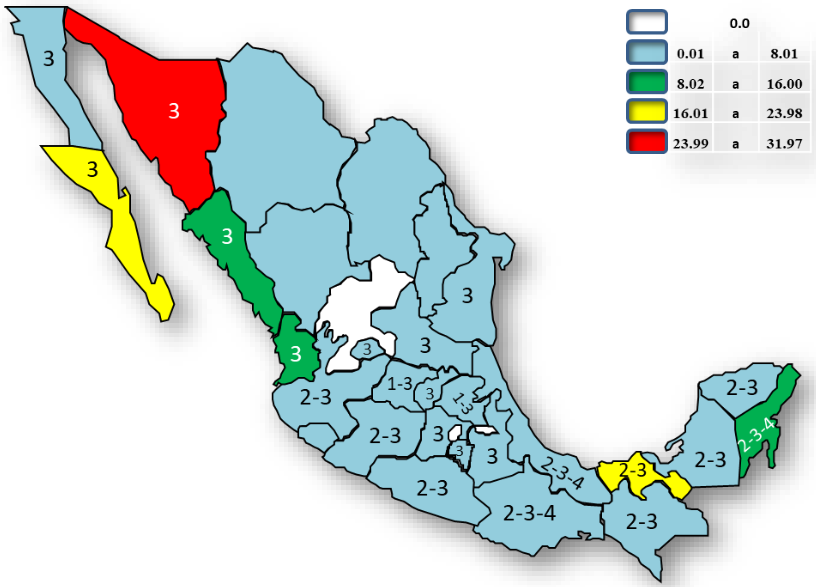
\includegraphics[width=9cm]{imagenes/Ant/mexico.png}
  \caption{Mapa de México con intervalos de incidencia de dengue y serotipos indicados por entidad. La imagen disponible no identifica el año ni la semana epidemiológica de corte.}
  \label{Fig:1.1}
\end{figure}


\begin{table}[htbp]
    \centering
    \caption{Cifras de dengue en México consignadas en el documento para 2025 y 2026. Fuente y semana de corte pendientes de verificación.}
    \label{tab:dengue_2025_2026}
    \small
    \setlength{\tabcolsep}{3pt}
    \begin{tabular}{|c|c|c|c|c|c|c|c|c|c|}
        \hline
        \multicolumn{2}{|c|}{\textbf{PROBABLES}} & \multicolumn{8}{c|}{\textbf{CONFIRMADOS}} \\
        \hline
        \textbf{2025} & \textbf{2026} & \multicolumn{4}{c|}{\textbf{2025}} & \multicolumn{4}{c|}{\textbf{2026}} \\
        \cline{3-10}
        & & \textbf{DNG} & \textbf{DCSA} & \textbf{DG} & \textbf{DCSA+DG} & \textbf{DNG} & \textbf{DCSA} & \textbf{DG} & \textbf{DCSA+DG} \\
        \hline
        49\,085 & 29\,977 & 2\,192 & 2\,167 & 175 & 2\,342 & 1\,230 & 1\,504 & 113 & 1\,617 \\
        \hline
    \end{tabular}
    \\[2mm]
    \raggedright \scriptsize \textbf{Abreviaturas:} \textbf{DNG:} Dengue No Grave; \textbf{DCSA:} Dengue Con Signos de Alarma; \textbf{DG:} Dengue Grave; \textbf{DCSA + DG:} DCSA + DG.
\end{table} 
\subsection{Estructura Genómica del Virus del Dengue (DENV)}
La caracterización genómica de cepas representativas de los cuatro serotipos del virus del dengue (DENV-1 a DENV-4) ha permitido comprender mejor la arquitectura viral y sus relaciones filogenéticas \textbf{véase la Figura \ref{fig:denv_secuencia}}. Los cuatro serotipos comparten aproximadamente un 70\% de identidad en su secuencia de aminoácidos. Asimismo, presentan un 50\% de homología con otros miembros representativos del género \textit{Flavivirus}, como el virus de la fiebre amarilla y el virus de la encefalitis japonesa \cite{arias1993dengue}.

\begin{figure}[H]
  \centering
  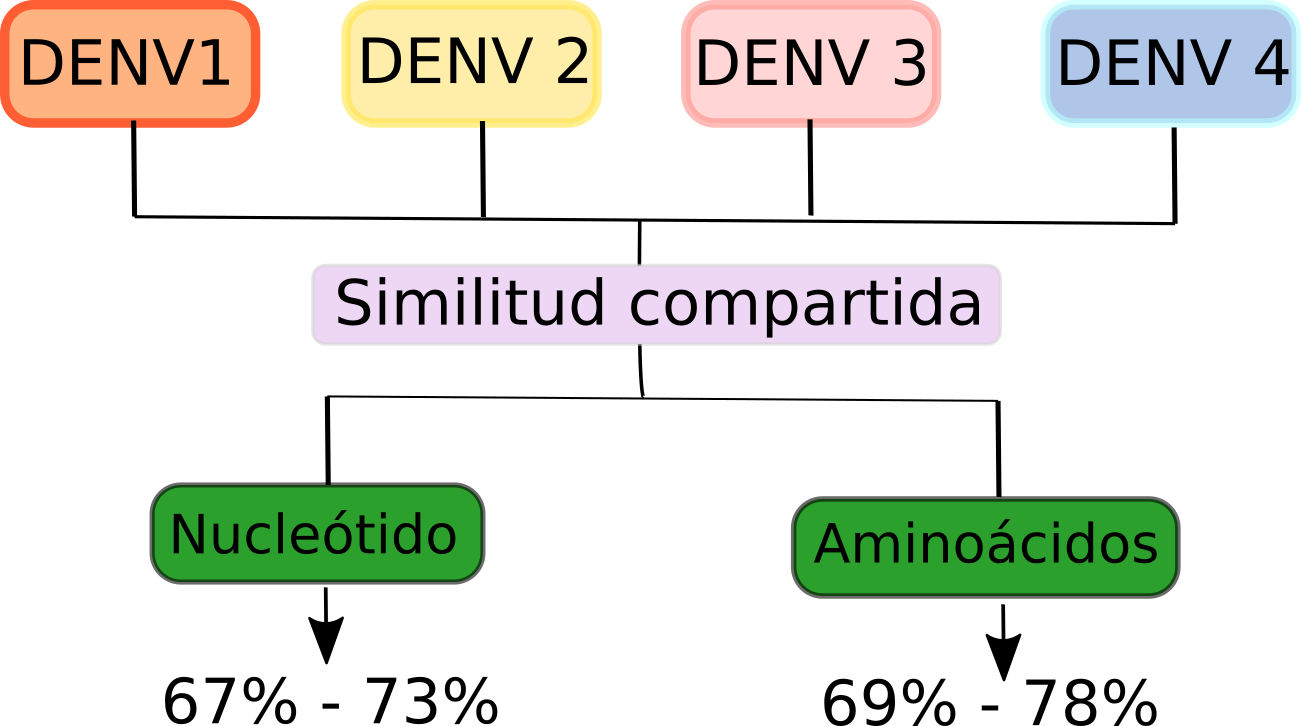
\includegraphics[width=9cm]{imagenes/Ant/diagrama-1.png}
  \caption{Relaciones de similitud de secuencia entre serotipos del DENV.}
  \label{fig:denv_secuencia}
\end{figure}

El genoma del virus del dengue está constituido por una molécula de ARN monocatenario de sentido positivo (+ssRNA), perteneciente a la familia \textit{Flaviviridae} \cite{sinha2024dengue}. Con una extensión aproximada de 11 kb, posee un único marco de lectura abierto (ORF) flanqueado por dos regiones no traducidas (5' UTR y 3' UTR). El extremo 5' UTR presenta una estructura de capuchón tipo 1 (m7GpppAmp). Por su parte, el extremo 3' UTR carece de la cola poli(A) convencional \cite{krishna2024dengue}.

La partícula viral madura posee una morfología esférica de aproximadamente 50 nm de diámetro. Esta estructura cuenta con una envoltura lipídica que rodea a la nucleocápside, dentro de la cual se empaqueta el ARN genómico \textbf{véase la Figura \ref{fig:denv_genoma}} \cite{dhole2024host}. Al ingresar a la célula hospedera, el ARN viral se traduce en la membrana del retículo endoplásmico (RE) en una poliproteína única. Posteriormente, esta cadena es procesada proteolíticamente para dar origen a tres proteínas estructurales —cápside (C), precursor de membrana/membrana (prM/M) y envoltura (E)— y a siete proteínas no estructurales (NS1, NS2A, NS2B, NS3, NS4A, NS4B y NS5) \cite{sinha2024dengue}.

\begin{figure}[H]
  \centering
  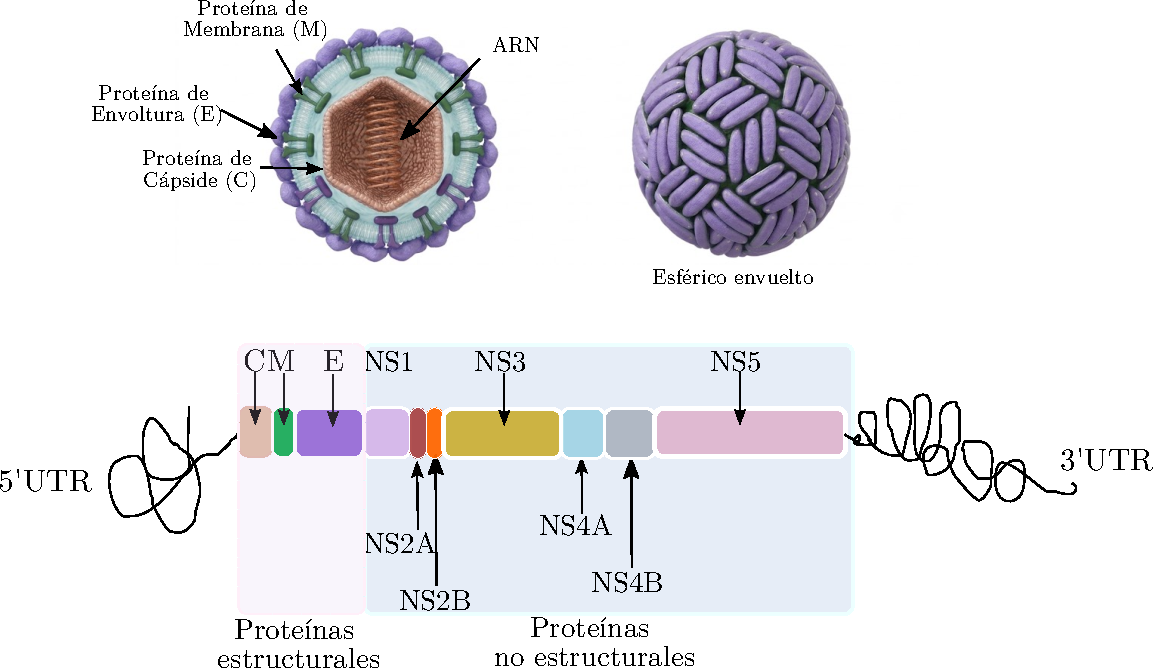
\includegraphics[width=13cm]{imagenes/Ant/genes.pdf}
  \caption{Organización genómica y procesamiento de la poliproteína del DENV.}
  \label{fig:denv_genoma}
\end{figure}

El procesamiento proteolítico co- y postraduccional de la poliproteína está coordinado por la proteasa viral NS2B-NS3 en el citoplasma, y por proteasas del huésped (señalasa y furina) en el lumen del RE. Las glicoproteínas E y M se organizan en la superficie de la bicapa lipídica con simetría icosaédrica. Durante el tránsito del virión inmaduro por la Red \textit{Trans}-Golgi (TGN), el pH ácido induce un cambio conformacional en la proteína E. Este cambio expone el sitio de escisión de prM para la acción de la furina. Posteriormente, la exocitosis hacia el espacio extracelular (pH $\approx 7.0$) provoca la liberación del péptido \textit{pr}. Este proceso permite la transición del virión desde una forma inmadura ("rugosa") hacia una partícula madura e infecciosa. Por su parte, las proteínas no estructurales cumplen funciones clave: NS1 evade la respuesta inmune al inhibir la activación del sistema del complemento, mientras que NS2A y NS4B participan en el ensamblaje del complejo de replicación \cite{pourzangiabadi2025dengue}.

\section{Arquitectura Molecular del Complejo Proteico NS2B-NS3}
La proteína no estructural 3 (NS3) es una enzima multifuncional constituida por dos dominios bien definidos. El dominio N-terminal actúa como una serina proteasa similar a la quimiotripsina, mientras que el dominio C-terminal presenta actividades de ARN helicasa, NTPasa y ARN 5'-trifosfatasa. Para llevar a cabo su función proteolítica, NS3 requiere de forma obligatoria interactuar en \textit{cis} o \textit{trans} con la proteína transmembrana NS2B, la cual actúa como su cofactor funcional \cite{diosa2020role}.

El dominio de serina proteasa comprende los primeros 180 aminoácidos N-terminales de NS3, de un total de 618 residuos. La expresión aislada de este dominio (NS3pro) o de la proteína completa (NS3 FL) produce agregados insolubles e inactivos. Para solubilizar y activar a NS3pro, se requiere la región hidrofílica central de NS2B (residuos 49 al 95). Mediante ingeniería de proteínas, la unión del segmento de NS2B con NS3pro a través de un enlazador flexible (Gly4-Ser-Gly4) permite obtener un complejo soluble y catalíticamente activo (NS2B-NS3pro). Al respecto, estudios estructurales de Erbel et al. (2006) demostraron que los residuos N-terminales 49–66 de NS2B actúan como una chaperona molecular. Esta región se inserta como una hebra $\beta$ en el barril N-terminal de NS3, protegiendo sus residuos hidrofóbicos de la exposición al solvente \cite{lescar2008towards}.

Sin embargo, la región N-terminal de NS2B no es suficiente para la actividad catalítica. Los residuos C-terminales del cofactor (Glu66–Leu95) son indispensables para estructurar el sitio activo. En esta zona, los aminoácidos Glu67–Asp76 forman las hebras $\beta_2$ y $\beta_3$. Por su parte, los residuos Arg78–Leu87 constituyen un bucle $\beta$ que abraza el barril C-terminal de NS3 \textbf{véase la Figura \ref{fig:ns2b_ns3_abierta}} . Esta disposición posiciona aminoácidos clave (Gly151, Gly153 y Tyr161) para el reconocimiento del sustrato e interviene directamente en la conformación de los bolsillos S2 y S3 \cite{erbel2006structural}. En consecuencia, el cofactor NS2B ejerce un doble papel regulador sobre NS3. Por un lado, estabiliza el plegamiento terciario del dominio proteasa. Por el otro, participa de forma directa en la conformación de la cavidad catalítica, permitiendo el reconocimiento de residuos básicos (Arg/Lys) en las posiciones P1 y P2 del sustrato \cite{luo2015flavivirus}.

Análisis estructurales comparativos revelan que, en ausencia de NS3pro, el cofactor NS2B libre se encuentra desordenado en solución. Al asociarse, la región N-terminal del cofactor forma un complejo estable con el dominio proteasa, mientras que su extremo C-terminal mantiene una alta flexibilidad. Estudios de cristalografía en estado \textit{apo} (libre de ligando) de flavivirus como el WNV y el DENV muestran que la proteasa existe principalmente en una ``conformación abierta'' inactiva. En este estado, la región C-terminal de NS2B se orienta hacia el solvente y permanece alejada del centro catalítico. Esta disposición espacial impide la catálisis, ya que se necesita la interacción directa de los residuos C-terminales del cofactor para organizar funcionalmente el sitio activo \cite{li2020insights}.

\begin{figure}[H]
  \centering
  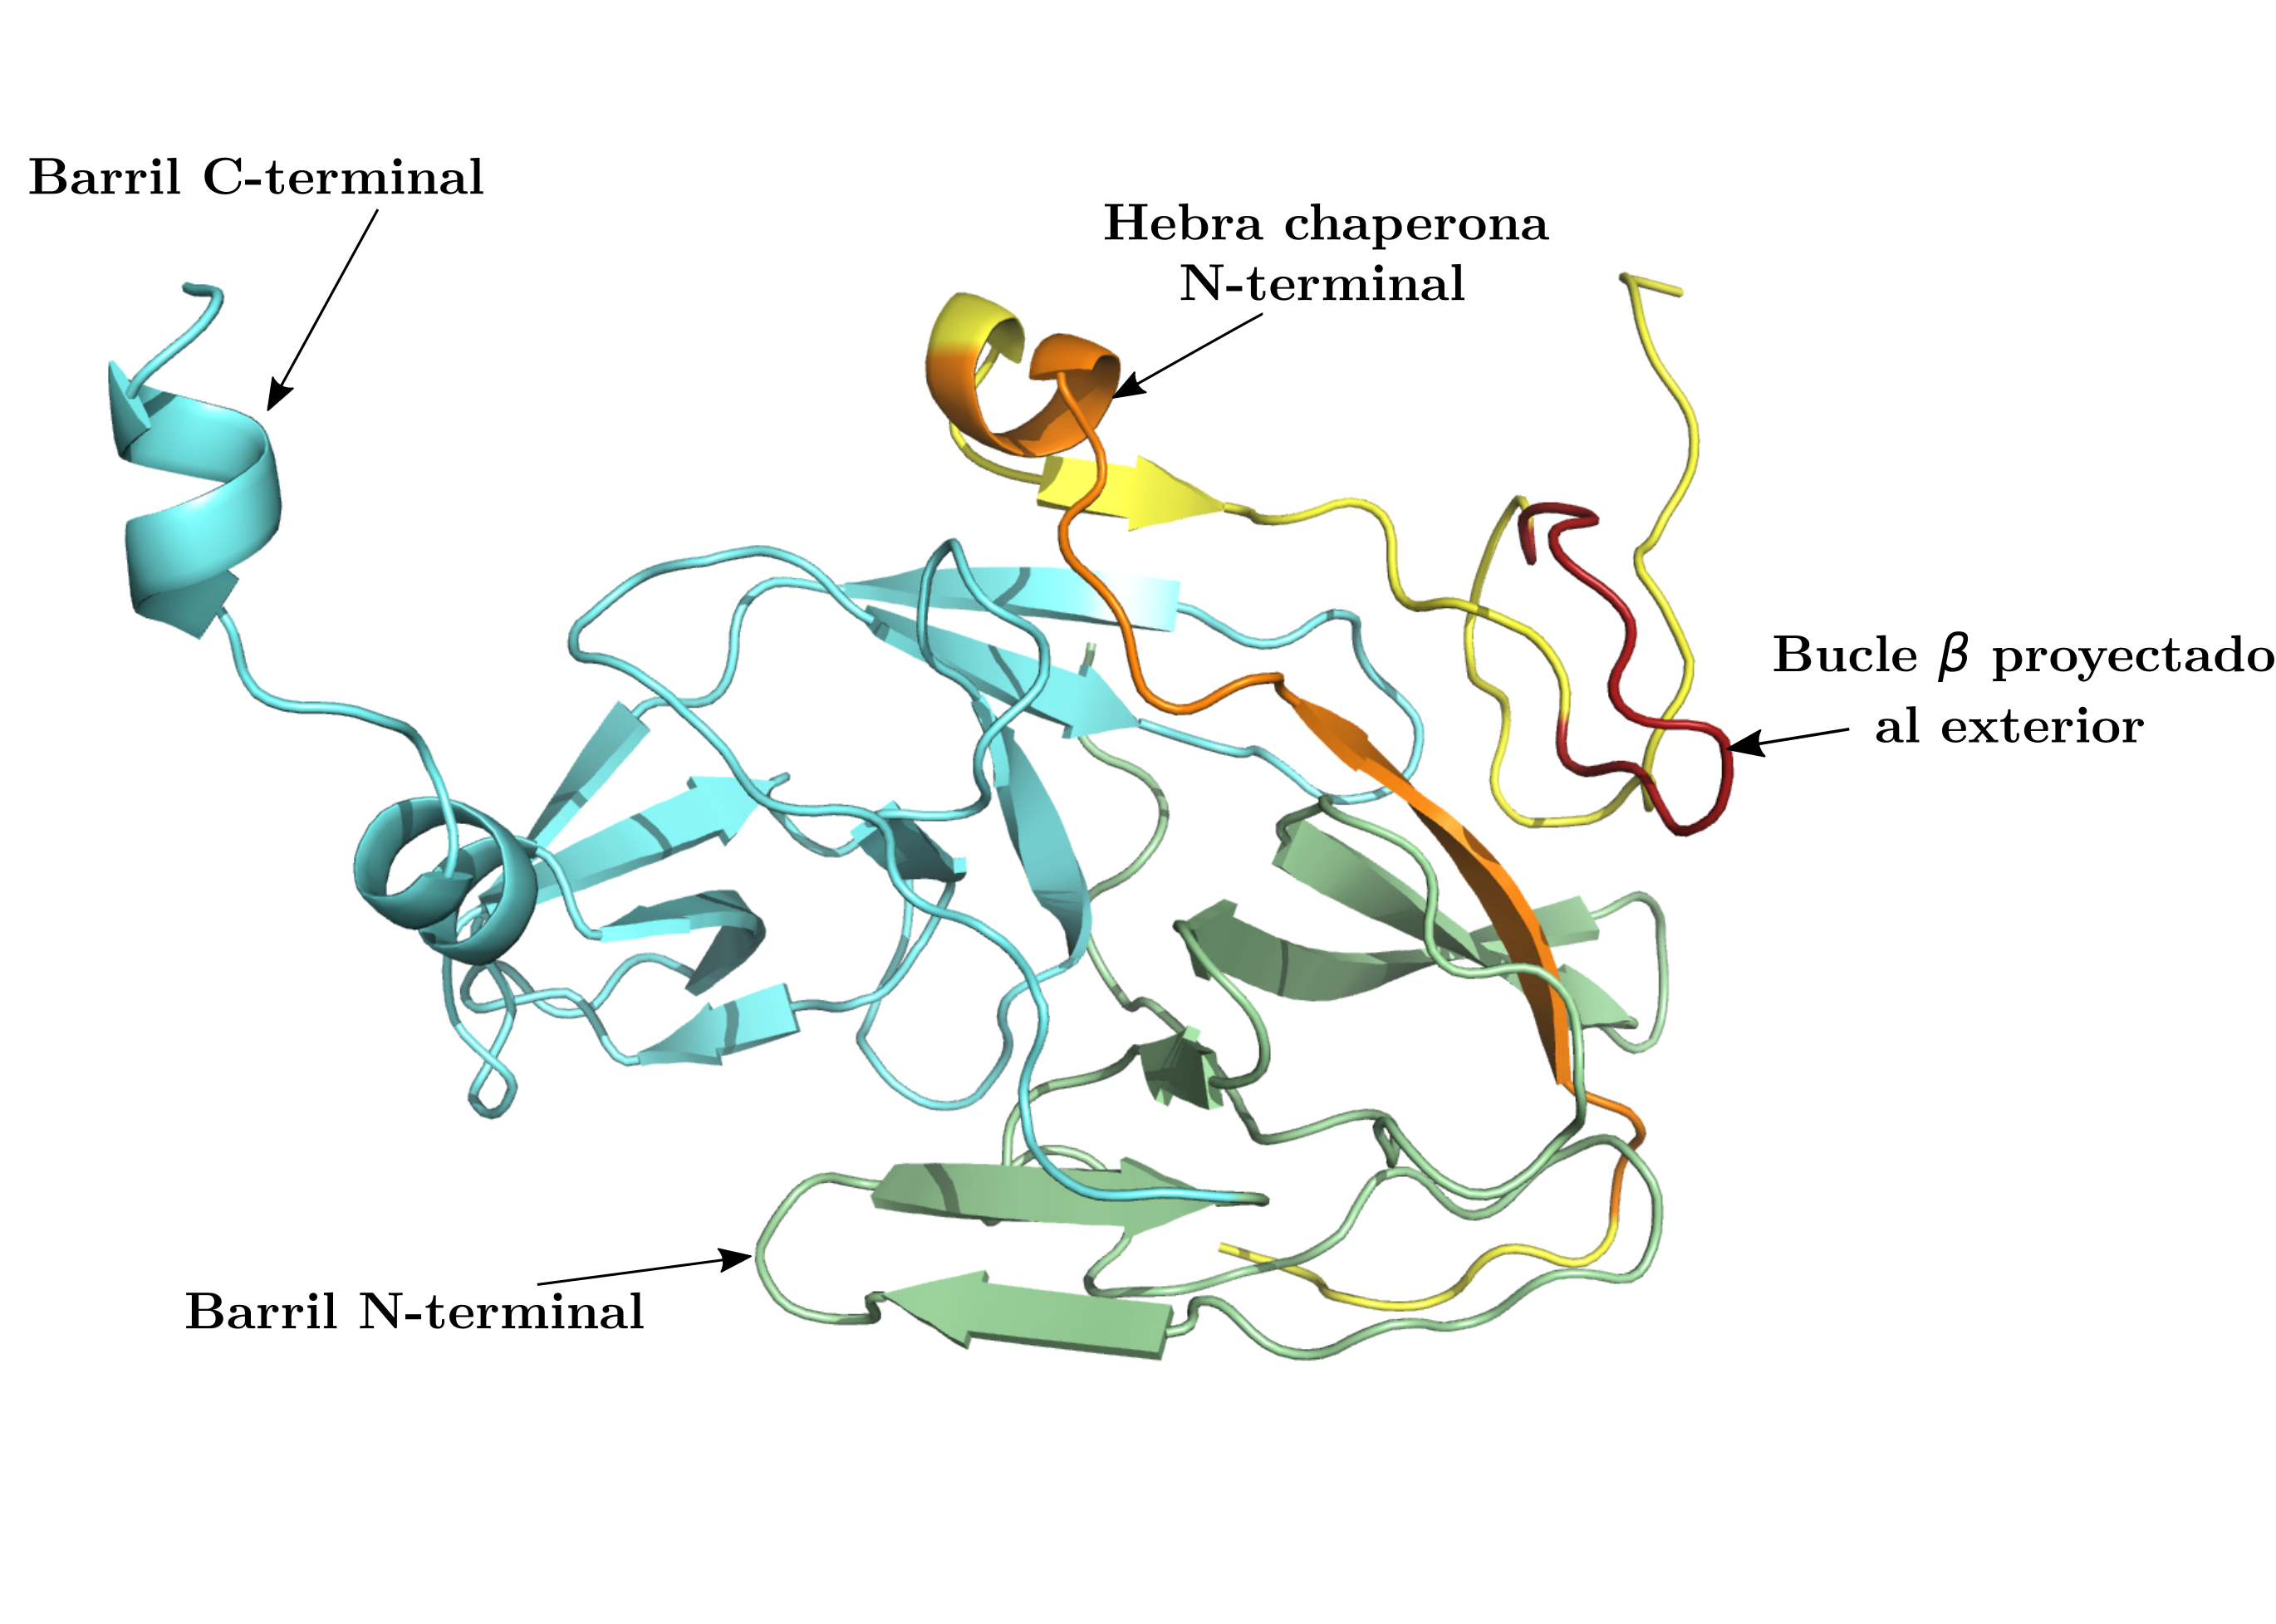
\includegraphics[width=13cm]{imagenes/Ant/2FOM-bucles.png}
  \caption{Estructura cristalina de la proteasa NS2B-NS3 del DENV-2 en conformación abierta (PDB ID: 2FOM). Representación tridimensional en cinta del complejo en ausencia de ligando. Se destacan los dos barriles $\beta$ (N-terminal y C-terminal) que forman el núcleo catalítico de NS3, la hebra chaperona N-terminal del cofactor NS2B anclada a NS3 y el bucle $\beta$ C-terminal proyectado hacia el exterior, característico del estado inactivo o desacoplado \cite{li2020insights,de2011binding,maus2021sar}.}
  \label{fig:ns2b_ns3_abierta}
\end{figure}
La transición desde la conformación abierta inactiva hacia la ``conformación cerrada'' activa ocurre mediante un reordenamiento conformacional. Este cambio es impulsado por la unión del sustrato o de un inhibidor ortostérico. Durante el proceso, el extremo C-terminal de NS2B se pliega alrededor de NS3pro, formando una horquilla $\beta$ que cubre la cavidad catalítica. Este cierre conformacional empaqueta los residuos clave del cofactor contra el dominio catalítico. De este modo, se fija la estructura tridimensional de los subsitios S2 a S4 y se activa la capacidad funcional del sitio catalítico \cite{li2020insights,de2011binding,maus2021sar}.
Es importante destacar que la conformación abierta observada en la estructura cristalina en estado \textit{apo} (PDB ID: 2FOM) ha sido objeto de debate en la literatura. Mientras que los estudios de cristalografía iniciales sugerían que la proteasa libre adopta preferentemente esta disposición inactiva, investigaciones de Resonancia Magnética Nuclear (RMN) en solución y análisis dinámicos recientes \cite{li2020insights,nitsche2023targeting} revelan que el complejo proteico experimenta una dinámica conformacional altamente fluida. En ausencia de ligando, la región C-terminal del cofactor NS2B oscila libremente entre un estado desacoplado y la conformación cerrada en un equilibrio termodinámico rápido, siendo la conformación cerrada la predominantemente poblada en condiciones fisiológicas. La cristalización de la forma abierta suele verse favorecida por empaquetamiento cristalino o por el uso de enlazadores artificiales de poliglicina ($G_4SG_4$). Por consiguiente, la captura de la estructura cerrada activa mediante RMN (PDB ID: 2M9P; \textbf{véase la Figura \ref{fig:ns2b_ns3_comparacion}}) evidencia que el dominio C-terminal de NS2B no solo actúa como un elemento estructural indispensable, sino como un regulador alostérico dinámico clave para la catálisis.



\begin{figure}[H]
  \centering
  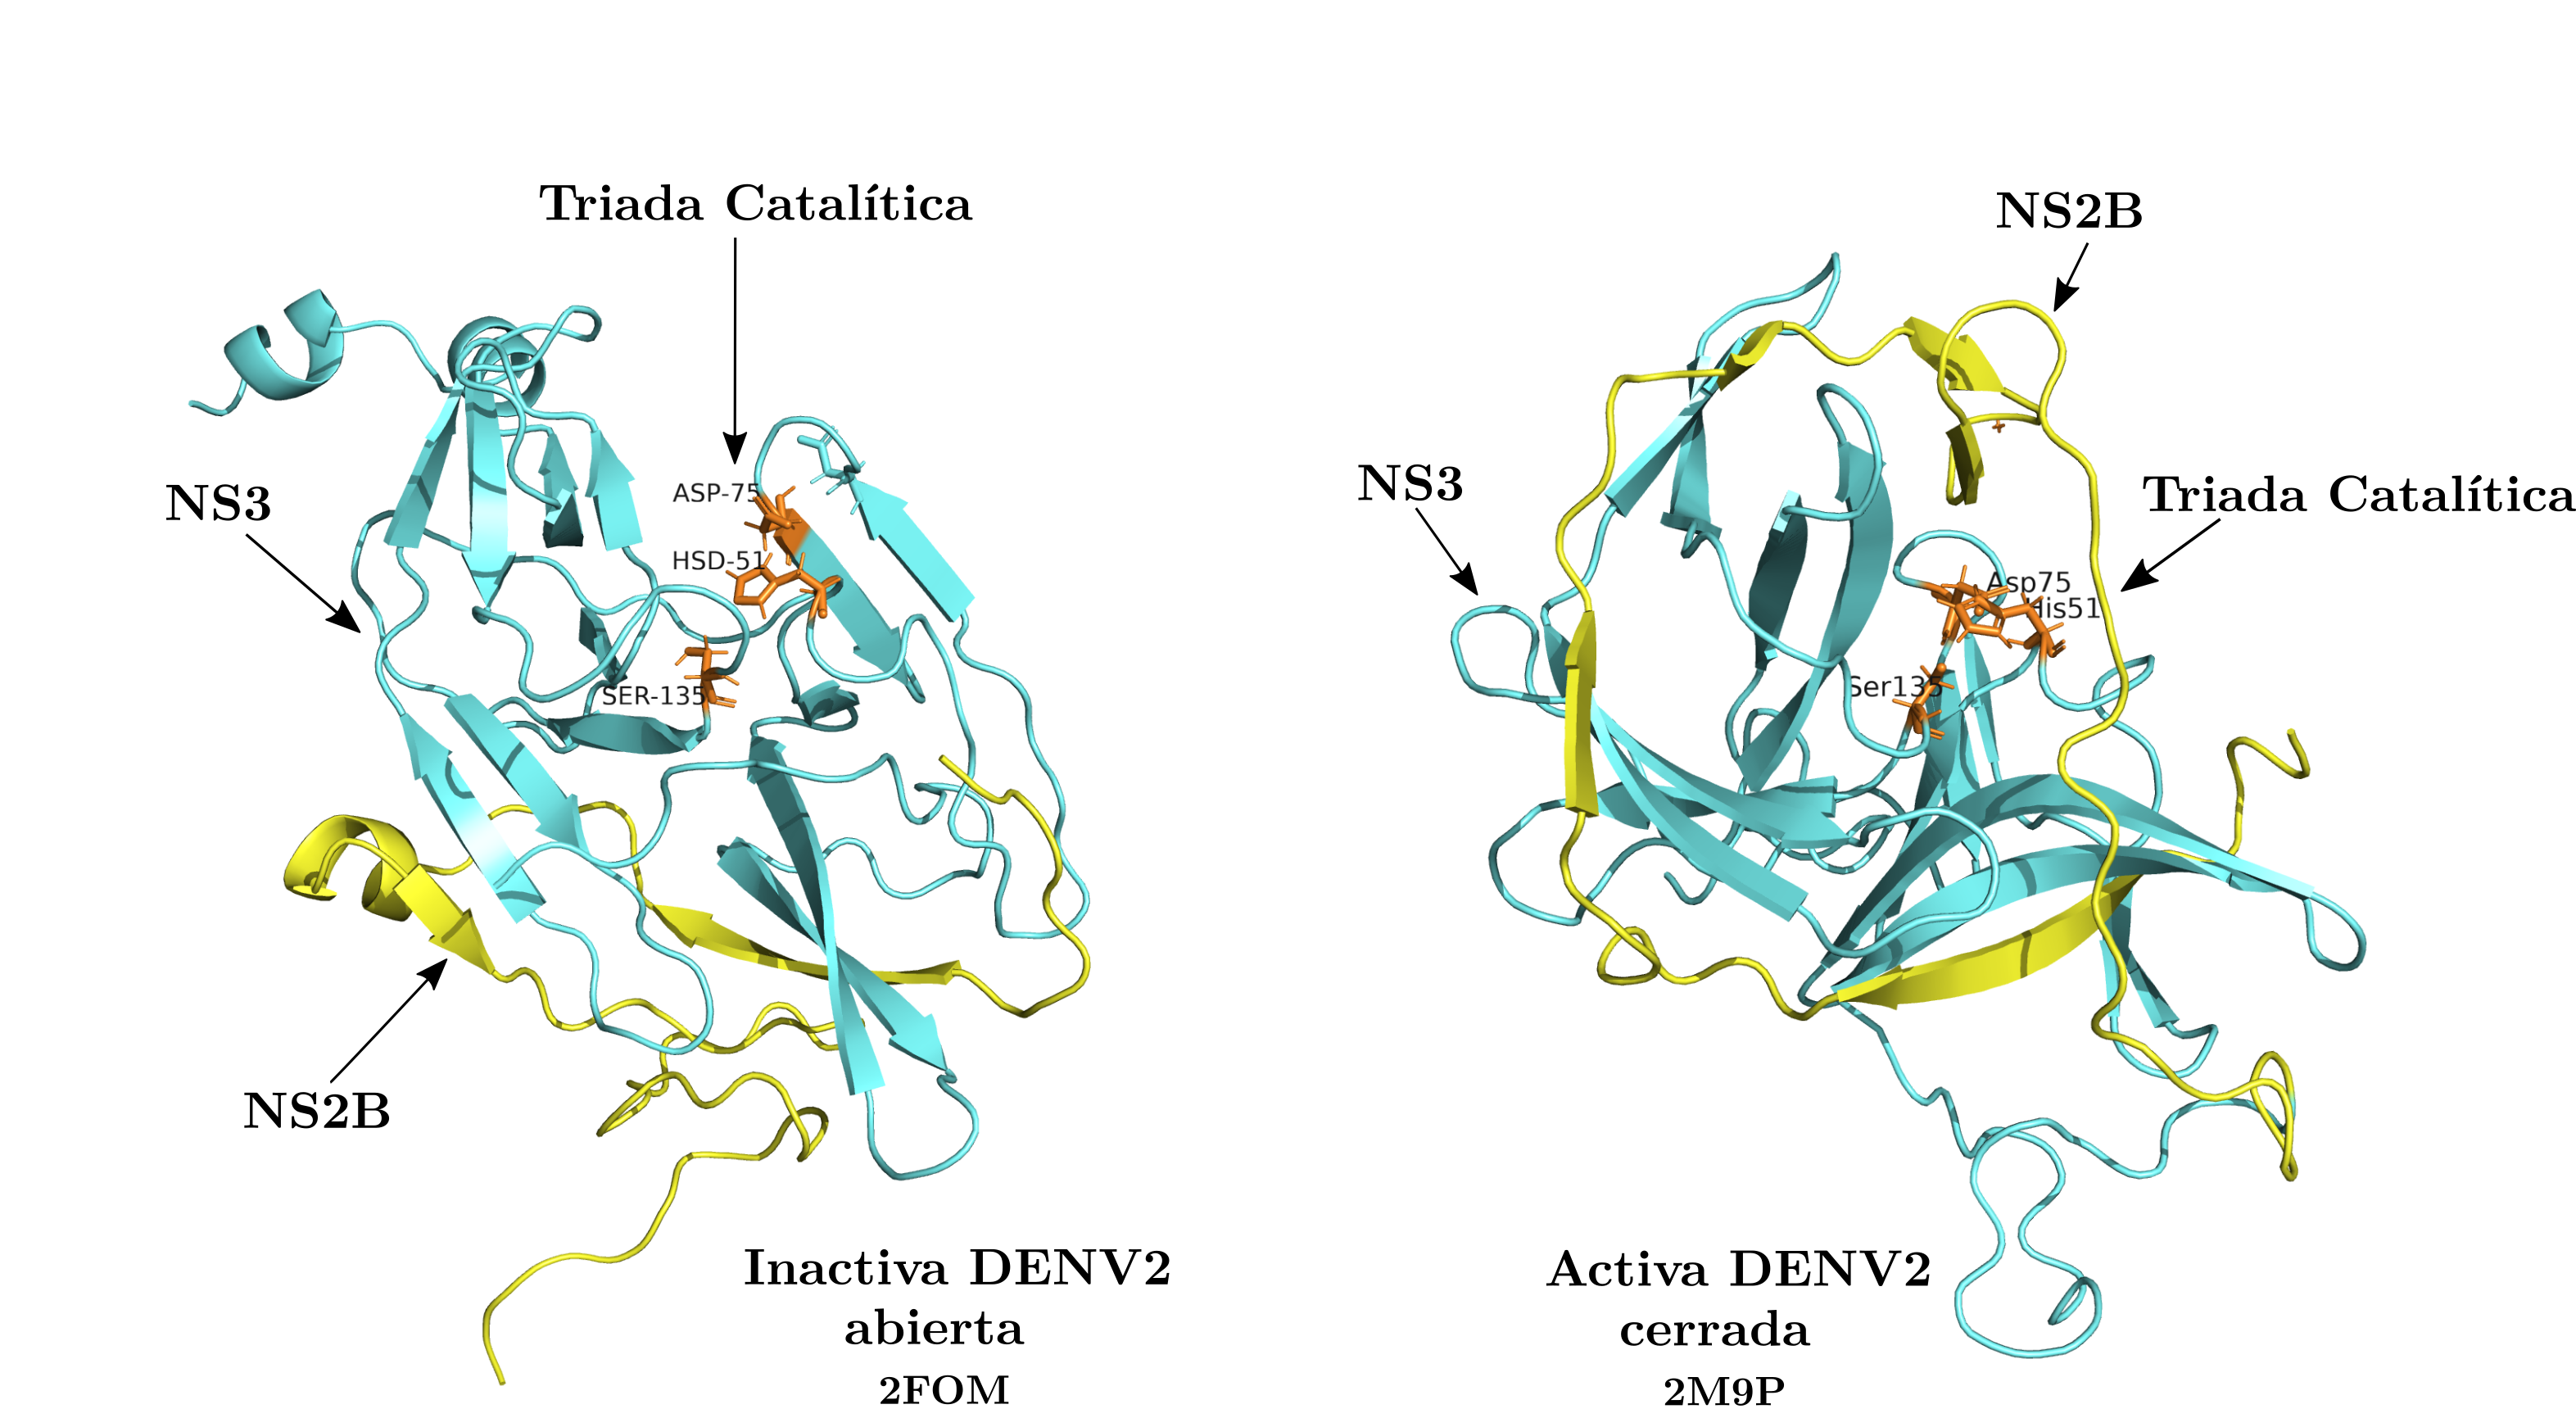
\includegraphics[width=16cm]{imagenes/Ant/2FOM-conformaciones.png}
  \caption{Comparación conformacional del complejo proteasa NS2B-NS3pro del virus del dengue serotipo 2 (DENV-2). \textbf{Izquierda:} Conformación abierta e inactiva en estado \textit{apo} (PDB ID: 2FOM). En esta forma, la región C-terminal del cofactor NS2B (amarillo) permanece desacoplada del dominio catalítico NS3 (cian). \textbf{Derecha:} Conformación cerrada y activa (PDB ID: 2M9P), la cual muestra el reordenamiento del bucle C-terminal de NS2B alrededor de NS3 para estructurar el sitio activo. En ambas estructuras se resaltan en bastones (\textit{sticks}) los residuos de la tríada catalítica (His51, Asp75 y Ser135) \cite{li2020insights,de2011binding,maus2021sar}.}
  \label{fig:ns2b_ns3_comparacion}
\end{figure}


\section{Mecanismo Catalítico e Inhibición Enzimática}
La maquinaria catalítica de la proteasa viral está formada por la tríada clásica de serina proteasas (His51, Asp75 y Ser135). Esta estructura se encuentra altamente conservada en la familia \textit{Flaviviridae}. Por su parte, la cavidad catalítica exhibe un potencial electrostático principalmente negativo. Esta propiedad es esencial, ya que condiciona la especificidad del sustrato al favorecer interacciones iónicas hacia residuos cargados positivamente (Lys y Arg) en los sitios de corte de la poliproteína \cite{li2020insights}.

La proteasa NS2B-NS3 constituye un blanco farmacológico primario debido a su papel en la replicación viral y en el procesamiento de factores inmunomoduladores del huésped. Su sitio activo se compone de ocho subsitios (S4, S3, S2, S1 | S1', S2', S3', S4') que reconocen la secuencia peptídica diana (P4, P3, P2, P1 | P1', P2', P3', P4'). Los subsitios S1–S4 poseen residuos ácidos que interaccionan preferentemente con aminoácidos catiónicos (Lys y Arg).

La catálisis opera mediante la tríada His51–Asp75–Ser135. En este proceso, el par Asp75–His51 desprotona el hidroxilo de Ser135, aumentando su nucleofilia para atacar el carbonilo del residuo P1. Este ataque genera un intermedio tetraédrico estabilizado por la cavidad del oxianión. Posteriormente, el colapso del intermedio libera el segmento peptídico P1'–P4' y forma un complejo acil-enzima. Finalmente, este se hidroliza por la adición de una molécula de agua catalítica, lo que regenera la enzima y libera el fragmento P1–P4  \cite{cavina2024orthoflaviviral}.

La delimitación estructural de los subsitios refleja un acoplamiento preciso entre NS3 y el cofactor NS2B. El bolsillo S1 está conformado por los residuos Asp129, Tyr130, Thr132, Tyr150 y Gly151 de NS3. En particular, la cadena lateral de Asp129 cumple una función idéntica a la de Asp189 en la tripsina, formando un par iónico indispensable para anclar la carga positiva de Arg/Lys en P1. Por su parte, el bolsillo S2 presenta una carga negativa aportada por los oxígenos carbonílicos de la cadena principal de NS2B. Allí, el residuo Asp152 de NS3 y la Gly83 de NS2B forman redes de puentes de hidrógeno para estabilizar el residuo básico en P2 \cite{li2020insights}.

El subsitio S1 está delimitado por Tyr161 (interacción catión-$\pi$) y Asp129 (par iónico con la Arg en P1). Los inhibidores de este complejo se clasifican en tres grupos: ortostéricos competitivos, ortostéricos no competitivos (por inducción de cambios conformacionales) y alostéricos no competitivos. Estos últimos se unen a regiones alejadas del sitio activo y evitan que NS2B adopte la conformación cerrada \cite{cavina2024orthoflaviviral}.

Por último, el dominio helicasa C-terminal de NS3 separa la doble hebra intermedia de ARN mediante la hidrólisis de ATP. Se ha demostrado que la actividad ATPasa de este dominio se estimula directamente por la presencia de ARN, lo que evidencia un acoplamiento alostérico funcional entre los centros catalíticos de la enzima \cite{lescar2008towards}.
\section{Mecanismos de Transmisión}
En el ámbito de la biología vectorial, las hembras de los mosquitos presentan hábitos hematófagos obligados. Por ello, requieren consumir sangre de huéspedes vertebrados para llevar a cabo la ovogénesis y la maduración de huevos viables. Estos vectores establecen sus hábitats dentro o en la periferia de las áreas habitables humanas, con picos de picadura concentrados en las primeras horas de la mañana y al atardecer. Asimismo, la puesta de huevecillos en recipientes con agua estancada y su gran cercanía a los hogares representan factores clave para la transmisión continua de la enfermedad \cite{fajardo2012dengue}.

El virus del dengue se transmite mediante la inoculación directa durante la picadura de un vector infectado, proceso conocido como transmisión horizontal. El mosquito adquiere el patógeno al alimentarse de la sangre de un individuo en fase de viremia. A partir de la ingesta, el virus se replica en el epitelio del intestino medio para luego diseminarse y colonizar las glándulas salivales del insecto \textbf{véase la Figura \ref{Fig:patologia_piel}}. Este lapso constituye el periodo de incubación extrínseca. Tras esta etapa, el vector es infectivo de forma permanente. Por el contrario, el tiempo transcurrido entre la inoculación viral en el ser humano y la aparición de los primeros síntomas se define como periodo de incubación intrínseco  \cite{salvadorgenetica}.

\begin{figure}[H]
  \centering
  \IfFileExists{imagenes/Ant/patologia.png}{
    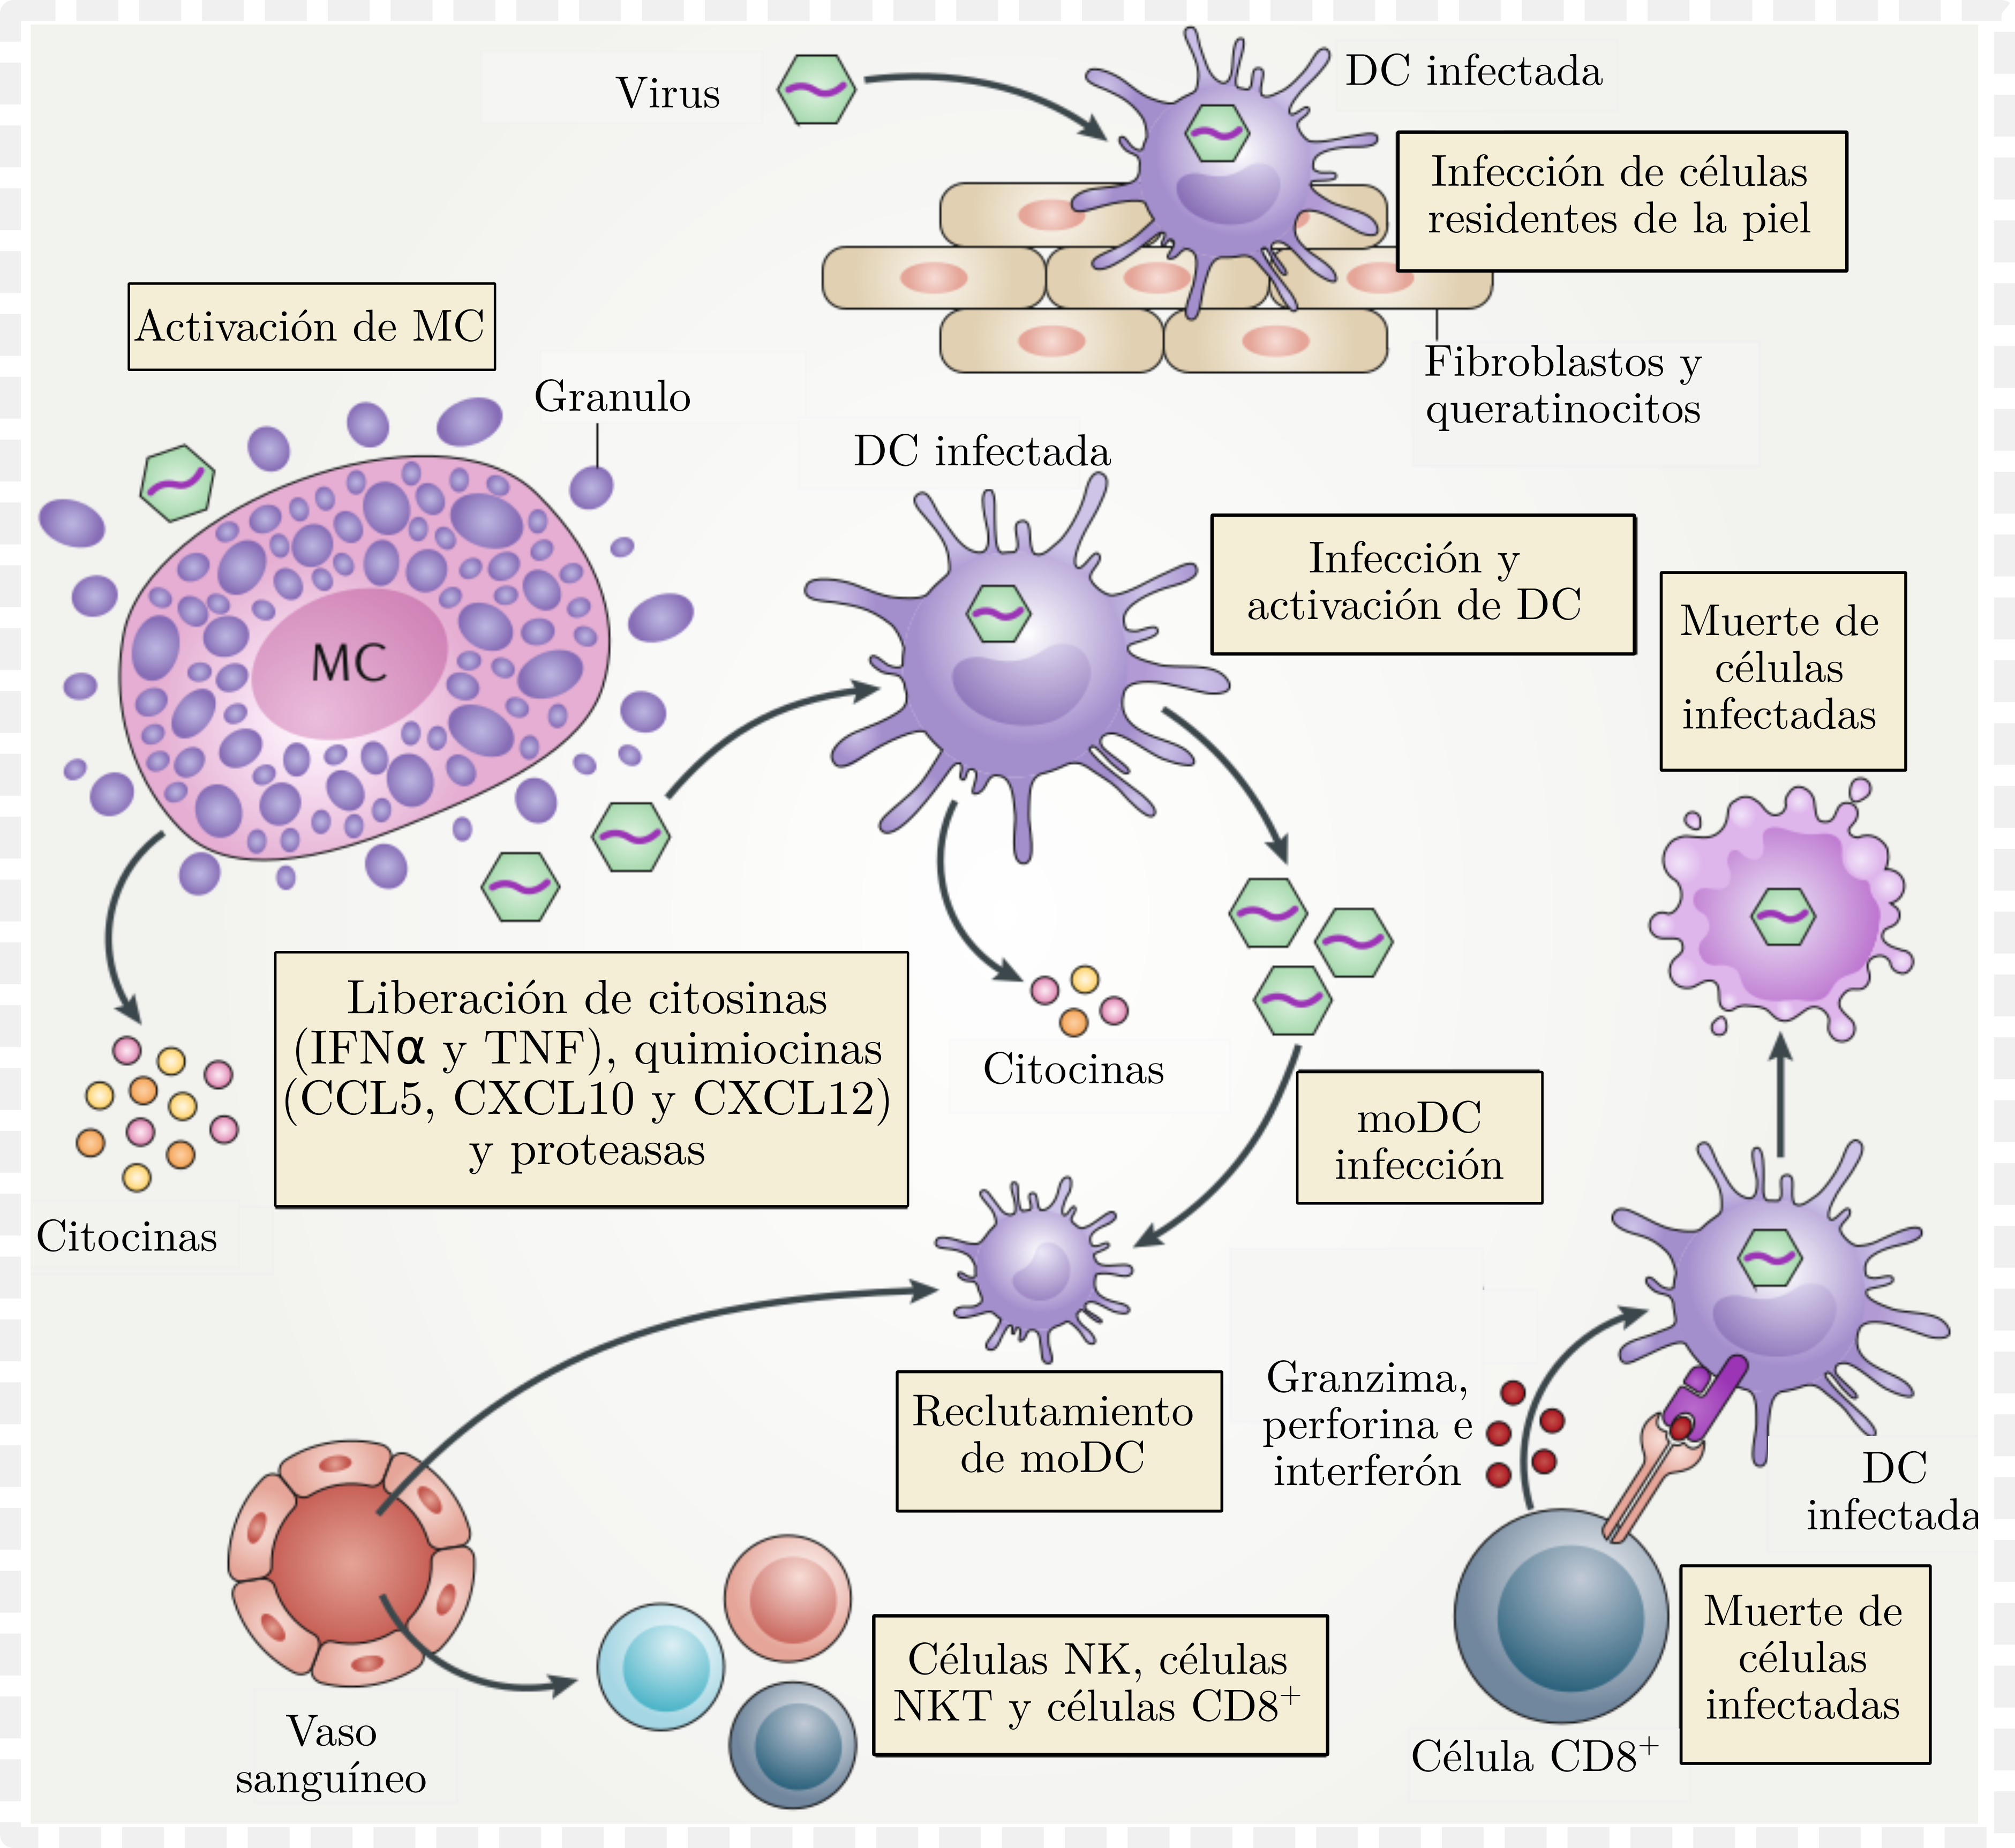
\includegraphics[width=0.7\textwidth]{imagenes/Ant/patologia.png}
  }{
    \framebox[0.75\textwidth]{\rule{0pt}{3.5cm} [Espacio reservado: Inmunopatología dérmica e interacción con células centinela]}
  }
  \caption{Fase inicial de la respuesta inmunológica local y activación de células centinela en la dermis tras la inoculación de DENV \cite{nanaware2021dengue}.}
  \label{Fig:patologia_piel}
\end{figure}

La inoculación del DENV ocurre cuando la hembra infectada de \textit{Aedes aegypti} deposita saliva contaminada en la piel del huésped durante la alimentación. Tras la replicación en los tejidos secundarios del vector, los viriones infecciosos se liberan en el microambiente cutáneo. Una vez en el organismo, el virus demuestra un amplio tropismo celular al interactuar con diversos receptores de superficie. Esta propiedad le permite infectar células epiteliales, fibroblastos, monocitos, macrófagos, células dendríticas, linfocitos B y T, células endoteliales y hepatocitos \cite{nanaware2021dengue}.

\section{Fisiopatología Local y Viremia Sistémica}
% Nota bibliográfica original pendiente de correspondencia: (10)
 En el sitio de inoculación dérmica, el DENV entra en contacto inmediato con las células centinela de la inmunidad innata. Entre ellas destacan las células de Langerhans (LC), las células dendríticas dérmicas (DC) y los mastocitos (MC). Los mastocitos detectan las partículas virales en cuestión de minutos y responden mediante una rápida desgranulación. Este proceso libera mediadores inflamatorios como interferón alfa (IFN-$\alpha$), factor de necrosis tumoral (TNF) y quimiocinas de atracción celular (CCL5, CXCL10 y CXCL12). A su vez, esta respuesta promueve el reclutamiento de linfocitos T citotóxicos CD8\textsuperscript{+}, células asesinas naturales (NK) y células NKT \textbf{(véase la Figura \ref{Fig:patologia_piel})}. No obstante, el virus infecta eficazmente a las células dendríticas y macrófagos residentes, utilizándolos como sitios primarios de replicación local. % Nota bibliográfica original pendiente de correspondencia: (10)

Las células dendríticas infectadas migran por los vasos linfáticos aferentes hacia los ganglios linfáticos regionales. En este punto, entran en contacto con nuevas poblaciones de macrófagos y monocitos a los cuales infectan. A partir de esta amplificación en el sistema linfoide, el virus se disemina por el torrente sanguíneo, originando una viremia sistémica. De esta manera, el patógeno logra colonizar órganos secundarios como el bazo, los riñones, los pulmones y el hígado. El estado virémico es detectable entre 24 y 48 horas antes del inicio de los síntomas y suele persistir de 10 a 12 días. Si un mosquito susceptible se alimenta durante este periodo, el ciclo biológico del virus se perpetúa \cite{nanaware2021dengue}.

La colonización de los ganglios linfáticos convierte a estas estructuras en centros de replicación viral masiva. Este paso resulta esencial para la consolidación de la viremia y para la subsecuente presentación de antígenos al sistema inmune adaptativo \cite{st2019adaptive}.

\section{Inmunopatología del Dengue Secundario}
 La efectividad de la respuesta inmune depende de la capacidad neutralizante de los anticuerpos dirigidos contra los dominios de la envoltura (E, prM/M) y la proteína no estructural NS1. Una infección primaria por un serotipo específico genera inmunidad permanente frente a ese mismo serotipo homotípico. Sin embargo, ante una infección secundaria por una cepa heterotípica, los anticuerpos preexistentes solo proporcionan una protección parcial y temporal. Por otro lado, la ARN polimerasa viral carece de actividad de corrección de pruebas, lo que otorga al DENV una elevada tasa de mutación y gran variabilidad antigénica. Estas variaciones permiten al virus escapar de la neutralización efectiva, desencadenando el fenómeno de Aumento Dependiente de Anticuerpos (ADE, por sus siglas en inglés).
La severidad de las manifestaciones clínicas está modulada tanto por factores virales (serotipo y mutaciones específicas) como por factores del huésped (edad y perfil inmunológico previo) \cite{dhole2024host}.

En el ámbito de la inmunidad celular, la proteína no estructural NS3 se considera el blanco inmunodominante para la respuesta de linfocitos T citotóxicos CD8\textsuperscript{+} y T colaboradores CD4\textsuperscript{+}. Sin embargo, la baja homología de secuencia entre los cuatro serotipos (entre el 50\% y el 60\%) limita la reactividad cruzada protectora. Durante una infección secundaria heteróloga (especialmente por el serotipo 2, DENV-2), los anticuerpos no neutralizantes forman inmunocomplejos con el virus. Estos complejos facilitan la entrada viral a monocitos y macrófagos a través de los receptores Fc$\gamma$R, incrementando exponencialmente la carga viral. Como consecuencia, se desencadena una liberación masiva de mediadores inflamatorios (tormenta de citocinas) y una activación inadecuada de las células T de memoria (Pecado Antigénico Original). Este proceso culmina en complicaciones graves como la fuga vascular, la fiebre hemorrágica por dengue y el síndrome de choque \textbf{véase la Figura \ref{Fig:inmunopatogenia_tikz}} \cite{st2019adaptive}.
\begin{figure}[H]
\centering
\resizebox{\textwidth}{!}{%
\begin{tikzpicture}[
    node distance=1.2cm and 1.0cm,
    primary/.style={rectangle, draw=blu1, fill=blu, text width=3.8cm, align=center, rounded corners, minimum height=1.2cm, thick},
    secondary/.style={rectangle, draw=red!70, fill=red!5, text width=3.8cm, align=center, rounded corners, minimum height=1.2cm, thick},
    arrow/.style={-Stealth, thick, draw=gray!80}
]

    % --- COLUMNA IZQUIERDA: INFECCIÓN PRIMARIA ---
    \node (prim) [primary] {\textbf{Infección Primaria} \\ Serotipo DENV-1};
    \node (cent) [primary, below=of prim, yshift=-0.3cm] {Infección de Centinelas \\ (DC, Macrófagos, MC)};
    \node (gl) [primary, below=of cent, yshift=-0.3cm] {Migración a Ganglios \\ Activación CD4\textsuperscript{+}, CD8\textsuperscript{+} y Ab};
    \node (res) [primary, below=of gl, yshift=-0.3cm, fill=green!5, draw=green!60] {\textbf{Enfermedad Autolimitada} \\ Aclaramiento viral};

    % Flechas Columna Izquierda
    \draw [arrow] (prim) -- (cent);
    \draw [arrow] (cent) -- (gl);
    \draw [arrow] (gl) -- (res);

    % --- COLUMNA DERECHA: INFECCIÓN SECUNDARIA ---
    \node (ade) [secondary, right=3.5cm of cent] {\textbf{1. Fenómeno ADE} \\ Ab previos no neutralizan $\rightarrow$ Entrada vía Fc$\gamma$R $\rightarrow$ $\uparrow$ Carga Viral};
    \node (pao) [secondary, right=1.0cm of ade] {\textbf{2. Pecado Antigénico} \\ T-memoria ineficaces $\rightarrow$ Tormenta de Citocinas};
    \node (sec) [secondary, above=1.2cm of ade, xshift=2.5cm] {\textbf{Infección Secundaria} \\ Serotipo Heterólogo (DENV-2)};
    \node (shock) [secondary, below=1.5cm of ade, xshift=2.5cm, fill=red!20, draw=red!90, text width=5.2cm] {\textbf{Enfermedad Grave} \\ Fuga Vascular y Síndrome de Choque};

    % Flechas Columna Derecha
    \draw [arrow] (sec) -- (ade);
    \draw [arrow] (sec) -- (pao);
    \draw [arrow] (ade) -- (shock);
    \draw [arrow] (pao) -- (shock);

\end{tikzpicture}
}
\caption{Inmunopatogenia comparativa del dengue: evolución clínica diferencial entre la infección primaria autolimitada y la infección secundaria grave.}
\label{Fig:inmunopatogenia_tikz}
\end{figure}

\section{Ciclo de Replicación Intracelular y Maduración Viral}
El ciclo de replicación celular del virus del dengue (DENV) constituye un proceso molecular dinámico y altamente coordinado que involucra la reorganización de los compartimentos membranosos del huésped, desde la internalización endocítica hasta la maduración proteolítica en la vía secretora \cite{uno2023dengue,stjohn2023dengue}. Durante esta cascada, la interacción de las proteínas virales con la maquinaria celular permite la síntesis del genoma y el ensamblaje de nuevas partículas infectivas \textbf{véase la Figura \ref{Fig:ciclo_replicacion}}. Las etapas fundamentales que componen este ciclo intracelular se describen a continuación:

\begin{figure}[H]
  \centering
  \IfFileExists{imagenes/Ant/ciclo.png}{
    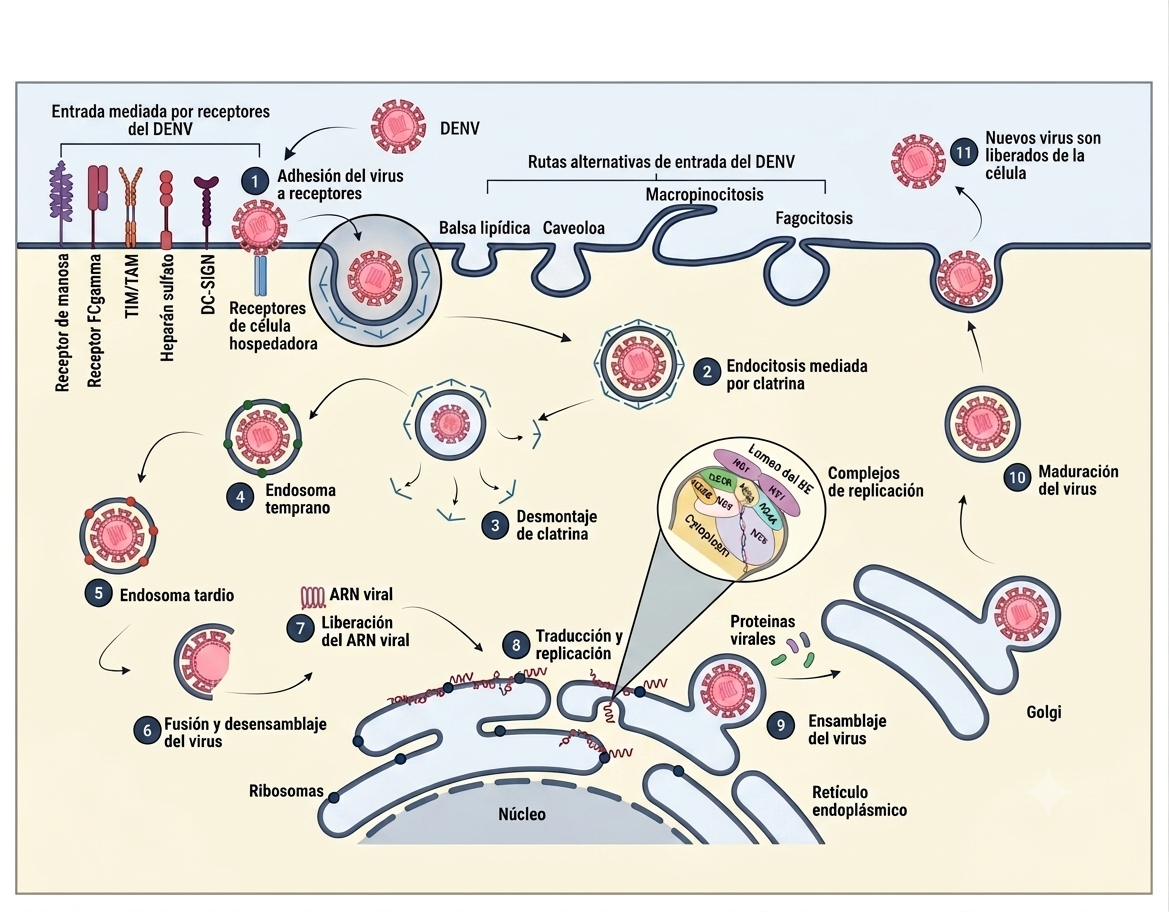
\includegraphics[width=0.85\textwidth]{imagenes/Ant/ciclo.png}
  }{
    \framebox[0.85\textwidth]{\rule{0pt}{5cm} [Espacio reservado: Esquema del ciclo de replicación celular del DENV]}
  }
  \caption{Representación esquemática del ciclo de replicación intracelular del virus del dengue (DENV).}
  \label{Fig:ciclo_replicacion}
\end{figure}

\begin{enumerate}
    \item \textbf{Adhesión celular e internalización:} La partícula viral se une a receptores de membrana específicos en la superficie de la célula hospedera, iniciando la internalización mediante endocitosis mediada por clatrina.
    \item \textbf{Formación de la vesícula endocítica:} El virión es reclutado en fosas revestidas de clatrina para constituir la vesícula de transporte interiorizada.
    \item \textbf{Desnudamiento del revestimiento:} Se produce la liberación de la cubierta de clatrina, dando paso a la maduración de la vesícula hacia un endosoma temprano.
    \item \textbf{Tránsito endosómico temprano:} El endosoma temprano, caracterizado por la presencia de la GTPasa Rab5, mantiene un pH aproximado de 6.5.
    \item \textbf{Acidificación endosómica tardía:} El endosoma madura a endosoma tardío (marcado por la proteína Rab7), donde la bomba de protones reduce el pH interno a valores cercanos a 5.5.
    \item \textbf{Fusión de membranas:} El entorno ácido induce cambios conformacionales en la glucoproteína E de la envoltura viral, desencadenando la fusión entre la membrana viral y la membrana endosómica.
    \item \textbf{Desensamblaje y liberación del genoma:} Se libera la nucleocápside al citosol celular, permitiendo la desagregación del genoma de ARN monocatenario de polaridad positiva (+ssRNA).
    \item \textbf{Traducción y replicación en el Retículo Endoplásmico (RE):} El ARN viral es traducido en el RE para sintetizar una poliproteína única que es procesada por proteasas virales (NS2B-NS3) y celulares. Las invaginaciones en la membrana del RE conforman los complejos de replicación.
    \item \textbf{Ensamblaje inmaduro:} El genoma replicado y las proteínas estructurales se ensamblan en la superficie del RE, brotando hacia el lumen celular como partículas virales inmaduras e inefectivas.
    \item \textbf{Maduración por Furina:} Los viriones inmaduros se transportan a través de la Red Trans-Golgi (TGN), donde la proteasa hospedera furina escinde la proteína prM, generando partículas virales maduras y potencialmente infectivas.
    \item \textbf{Exocitosis:} Los viriones maduros son liberados al espacio extracelular mediante vesículas secretoras, completando el ciclo de infección e iniciando la propagación sistémica \cite{screaton2015new}.
\end{enumerate}

\section{Estrategias de Inhibición de la Proteasa NS2B-NS3 en DENV-2}
Existen determinadas familias químicas de inhibidores de la proteasa \textbf{NS2B-NS3 de DENV-2}, debido a que la proteasa heterodimérica NS2B-NS3 de DENV-2 es un blanco terapéutico esencial para el desarrollo de antivirales. Para su procesamiento proteolítico, la enzima fluctúa entre dos conformaciones principales: una \textbf{conformación abierta (inactiva)}, donde la región C-terminal del cofactor NS2B está desordenada o libre, y una \textbf{conformación cerrada (activa)}, en la que NS2B envuelve al dominio proteasa NS3 formando un cinturón $\beta$ que completa el sitio activo \cite{chandramouli2010serotype, maus2021sar}.

A partir de esta dinámica estructural, se han desarrollado diversas familias de inhibidores que actúan mediante distintos mecanismos de acción:

\vspace{0.5em}

\subsection{Inhibidores alostéricos derivados de quinoxalina}
Esta clase de compuestos no competitivos posee un núcleo central de quinoxalina. En la posición 2 presenta una fracción de amina cíclica (como prolina, pirrolidina o piperidina), mientras que las posiciones 3 y 7 contienen diversos sustituyentes lipofílicos.

\begin{itemize}
    \item \textbf{Mecanismo de acción:} Se unen a un bolsillo alostérico situado en el lado opuesto de la tríada catalítica. Esta interacción bloquea la transición de la enzima hacia su forma activa (cerrada). De esta manera, se impide que el cofactor NS2B se asocie correctamente con el dominio NS3 \cite{zephyr2023allosteric}.
    \item \textbf{Residuos de interacción en DENV-2:} La cavidad alostérica está definida por los residuos \textbf{Gln74, Trp83, Ile123, Asn152 y Val155} en NS3. Al respecto, experimentos con ``trampas de disulfuro'' (entre \textbf{Lys117} en NS3 y \textbf{Ser75} en NS2B) confirmaron que estos inhibidores pierden eficacia cuando la proteína queda atrapada en su forma cerrada. Este hallazgo demuestra la superposición entre su sitio de acción y la interfaz de unión de NS2B.
    \item \textbf{Compuestos destacados y potencia:}
    \begin{itemize}
        \item \textbf{Compuesto 32} (análogo de piperidina con grupo guanidinio): $\text{IC}_{50} = 130 \pm 9\ \mu\text{M}$ (enzimático); $\text{EC}_{50} = 2.7\ \mu\text{M}$ (celular, el más potente en ensayos celulares contra DENV-2).
        \item \textbf{Compuesto 19} (análogo de pirrolidina): $\text{IC}_{50} = 160 \pm 8\ \mu\text{M}$.
        \item \textbf{Compuestos 33 y 36}: Derivados con notable potencia antiviral celular ($\text{EC}_{50} = 4.6\ \mu\text{M}$ y $4.4\ \mu\text{M}$, respectivamente) \cite{zephyr2023allosteric}.
    \end{itemize}
\end{itemize}
\subsection{Inhibidores Alostéricos (Benzotiazol y Benzofurano)}

Esta serie de compuestos no competitivos fue diseñada para unirse al bolsillo alostérico adyacente al residuo \textbf{Asn152}. Este aminoácido actúa como un \textbf{``interruptor molecular''} ubicado entre la cavidad activa y la alostérica. De este modo, regula la transición entre la conformación abierta e inactiva de la enzima.

\begin{itemize}
    \item \textbf{Mecanismo de acción:} Estabilizan la proteasa en su conformación abierta e inactiva mediante inhibición no competitiva. Al respecto, estudios de mutagénesis con cisteína única (mutante T122C y bloqueo con N-bencilmaleimida) confirmaron que estos inhibidores se ubican cerca del residuo \textbf{Thr122} y del bucle de los residuos 120s.
    \item \textbf{Residuos de interacción en DENV-2:} El farmacóforo clave (motivo catecol 5,6-dihidroxi) forma una red conservada de puentes de hidrógeno con \textbf{Lys74, Gly148 y Asn152}. Asimismo, interacciona con residuos del bolsillo lipofílico como \textbf{Met49, Leu76, Trp83, Lys84, Leu85, Glu86, Glu88, Trp89, Val146, Val147, Leu149, Ala164, Ile165 e Ile166}.
    \item \textbf{Compuestos destacados y potencia:}
    \begin{itemize}
        \item \textbf{Compuesto 34e (Derivado de Benzofurano):} Reemplaza el núcleo de benzotiazol mediante \textit{scaffold hopping}. La geometría ligeramente inclinada del benzofurano favorece la interacción entre el carbonilo de la amida y la \textbf{Lys74} de DENV-2. Esto le permite alcanzar una elevada potencia enzimática con un valor de $\text{IC}_{50} = 0.69 \pm 0.16\ \mu\text{M}$ ($0.73 \pm 0.015\ \mu\text{M}$ en el mutante T120A/N167Q).
        \item \textbf{Compuesto 25b (Benzotiazol truncado con yodo en \textit{para}):} Diseñado para maximizar la eficiencia de ligando ($\text{LE} = 0.41$). Presenta una $\text{IC}_{50} = 4.38 \pm 0.38\ \mu\text{M}$ ($K_i = 7.67\ \mu\text{M}$) contra DENV-2 y una marcada actividad en replicones virales celulares. En este caso, el átomo de yodo orientado hacia \textbf{Glu86/Glu88} favorece una interacción carboxilato-halógeno altamente efectiva.
        \item \textbf{Compuesto 23b (Estructura en forma de ``Y'', derivado del ácido 2,2-difenilacético):} Muestra una $\text{IC}_{50} = 11.12 \pm 0.49\ \mu\text{M}$ contra DENV-2. Fue diseñado para abarcar de forma simultánea las dos subcavidades hidrofóbicas que ocupan los enantiómeros de prolina. Su prodroga dimetoxilada (\textbf{22b}) logró reducir significativamente la replicación celular del ARN de DENV-2 gracias a una mayor permeabilidad de membrana \cite{maus2021sar}.
    \end{itemize}
\end{itemize}

\subsection{Inhibidores Ortostéricos y Modulación Mecánica (Rigidificación)}

\begin{itemize}
    \item \textbf{Inhibidores Competitivos Ortostéricos:} Se dirigen directamente a la cavidad del sitio activo unida a la tríada catalítica (\textbf{His51, Asp75, Ser135}).
    \begin{itemize}
        \item \textit{Limitación principal:} El sitio activo de la proteasa flaviviral es muy superficial y cargado negativamente, mostrando preferencia por residuos dibásicos en las posiciones $P1$ y $P2$. Los miméticos del sustrato suelen presentar propiedades farmacocinéticas deficientes y una pobre permeabilidad a través de las membranas celulares.
    \end{itemize}
    \item \textbf{Estrategia de Rigidificación (Efecto Alostérico Mecánico):} Propuesta a partir de la identificación del tramo de 10 residuos en NS3 (residuos 11 al 20). Dado que la proteasa requiere flexibilidad estructural para llevar a cabo la catálisis, los ligandos que reducen o rigidizan la movilidad de la enzima disminuyen drásticamente su eficiencia catalítica ($V_{\max}$) sin alterar necesariamente la capacidad de unión al sustrato ($K_m$)\cite{chandramouli2010serotype}.
\end{itemize} \newpage

\subsection{Comparación de inhibidores de la proteasa NS2B-NS3}
La Tabla~\ref{tab:inhibidores} resume los compuestos y las estrategias descritas.
\begingroup
\scriptsize % Tamaño de letra adaptado para 6 columnas
\setlength{\tabcolsep}{1.5pt} % Espaciado lateral de seguridad entre columnas
\begin{xltabular}{\textwidth}{
  >{\hsize=0.9\hsize\RaggedRight\arraybackslash}X
  >{\hsize=0.7\hsize\RaggedRight\arraybackslash}X
  >{\hsize=1.1\hsize\RaggedRight\arraybackslash}X
  >{\hsize=1.1\hsize\RaggedRight\arraybackslash}X
  >{\hsize=1.1\hsize\RaggedRight\arraybackslash}X
  >{\hsize=1.1\hsize\RaggedRight\arraybackslash}X
}
\caption{Resumen de inhibidores y sitios de unión.} \label{tab:inhibidores} \\ % <--- CAPTION
\toprule
\textbf{Familia /\allowbreak Compuesto} & \textbf{Sitio de Unión} & \textbf{Regiones y Residuos Clave (DENV-2)} & \textbf{Eficacia /\allowbreak Potencia Reportada} & \textbf{Importancia Estratégica} & \textbf{Limitaciones Principales} \\
\midrule
\endhead

\bottomrule
\endfoot

\textbf{Quinoxalinas} \newline (\textit{Comp. 32, 19, 33, 36}) & \textbf{Alostérico} \newline (Interfaz distal) & \textbf{NS3:} Q74, W83, I123, N152, V155 \newline \textbf{Evidencia:} K117 (NS3) y S75 (NS2B) [trampa disulfuro] & \textbf{Comp. 32:} \newline $\text{IC}_{50} = 130 \pm 9\ \mu\text{M}$ \newline $\text{EC}_{50} = 2.7\ \mu\text{M}$ \newline \textbf{Comp. 19:} \newline $\text{IC}_{50} = 160 \pm 8\ \mu\text{M}$ & Desplaza al cofactor NS2B e impide que la proteasa pase de la forma abierta a la cerrada activa. & Pobre correlación entre baja potencia enzimática in vitro y alta eficacia en ensayos celulares. Escasez de estructuras cristalinas en complejo. \\
\midrule
\textbf{Benzofurano 34e} & \textbf{Alostérico} \newline (Cercano a N152)& \textbf{NS3:} K74 (interacción mejorada con carbonilo), G148, N152 (motivo catecol)& $\text{IC}_{50} = 0.69 \pm 0.16\ \mu\text{M}$ \newline ($0.73 \pm 0.015\ \mu\text{M}$ en mutante T120A/\allowbreak N167Q) & Reemplazo por benzofurano adapta mejor la geometría a Lys74 de DENV-2, eliminando preferencia por ZIKV. & Reducida eficacia en replicación celular de DENV-2 atribuida a permeabilidad o metabolismo celular \cite{maus2021sar}. \\
\midrule
\textbf{Benzotiazol Truncado 25b} \newline (\textit{p-yodobenzamida}) & \textbf{Alostérico} \newline (Entrada al bolsillo alostérico) & \textbf{NS3:} K74, G148, N152 \newline \textbf{Residuos ácidos:} E86, E88 (contacto con yodo) & $\text{IC}_{50} = 4.38 \pm 0.38\ \mu\text{M}$ \newline $K_i = 7.67\ \mu\text{M}$\newline Disminución significativa de replicación de ARN celular & Excelente eficiencia de ligando ($\text{LE} = 0.41$). Interacción halógeno-carboxilato con Glu86/88 incrementa afinidad. & Requiere grupo dihidroxi (catecol) libre para actividad enzimática directa, sensible a oxidación in vitro \cite{maus2021sar}. \\
\midrule
\textbf{Inhibidores en ``Y''} \newline (\textit{Compuesto 23b}) & \textbf{Alostérico} \newline (Subbolsillos hidrofóbicos) & \textbf{NS3:} Subcavidades definidas por W89, A166, V146, V147 y N152 & $\text{IC}_{50} = 11.12 \pm 0.49\ \mu\text{M}$ \newline \textbf{Prodroga 22b:} Inhibición marcadamente potente en replicones & Ocupa simultáneamente las dos subcavidades lipofílicas exploradas por enantiómeros de prolina. & Restricción geométrica de la estructura en Y puede distorsionar la alineación del motivo catecol \cite{maus2021sar}. \\
\midrule
\textbf{Derivado de Panduratin A} \newline (\textit{Compuesto 246DA}) & \textbf{Ortostérico} \newline (Sitio activo) & \textbf{NS3:} Tríada catalítica (H51, D75, S135) \newline \textbf{Bolsillo hidrofóbico:} L76, W83, I165, I166 & $K_i = 19.84\ \mu\text{M}$ \newline Energía de complexación: $-76.8\ \text{kcal/mol}$ & Inhibidor competitivo no peptídico derivado de producto natural; establece múltiples puentes de H con la tríada catalítica. & Diseño y evaluación basados en acoplamiento molecular y química computacional; requiere validación biológica adicional \cite{frimayanti2011design}. \\
\midrule
\textbf{Análogos de Sustrato} & \textbf{Ortostérico} \newline (Sitio activo) & \textbf{NS3:} Tríada catalítica (H51, D75, S135) y bolsillos $P1/\allowbreak P2$ & Variable (alta afinidad in vitro en péptidos optimizados)& Bloqueo directo del centro catalítico primario, región conservada entre serotipos. & Farmacocinética muy deficiente y mala permeabilidad debido a cargas dibásicas en P1/\allowbreak P2 \cite{cavina2024orthoflaviviral}. \\
\midrule
\textbf{Rigidificación} & \textbf{Alostérico /\allowbreak Mecánico} & \textbf{NS3:} Tramo regulador de 10 aminoácidos (residuos 11 al 20 en NS3pro) & Modulación de la velocidad máxima ($V_{\max}$) sin alterar $K_m$ & Elimina la flexibilidad estructural necesaria para la catálisis; estrategia de amplio espectro. & Requiere diseñar moléculas pequeñas que restrinjan la dinámica sin depender del sitio activo \cite{chandramouli2010serotype}. \\
\end{xltabular}
\endgroup




\section{Manifestaciones Clínicas}
La infección sintomática por el virus del dengue presenta un periodo de incubación de 3 a 10 días. Su evolución se describe en tres fases clínicas, aunque no todos los pacientes desarrollan complicaciones en la fase crítica \cite{cdc2024dengueclinical}. La \textbf{fase febril} (2 a 7 días) inicia de forma súbita con fiebre alta, frecuentemente bifásica. Esta etapa se acompaña de cefalea, dolor retroorbitario, mialgias, artralgias, exantema cutáneo y síntomas gastrointestinales. A continuación acontece la \textbf{fase crítica} (habitualmente 24 a 48 horas), la cual coincide con la defervescencia. Esta fase se caracteriza por un aumento en la permeabilidad vascular, fuga plasmática, hemoconcentración y trombocitopenia, lo que conlleva un elevado riesgo de hemorragias y choque. Finalmente, la \textbf{fase de recuperación} (2 a 3 días) se distingue por la reabsorción del líquido extravascular, la estabilización hemodinámica y el retorno del apetito \cite{contreras2021aspectos, roquefactores}.

El desarrollo de formas graves de la enfermedad (dengue grave y síndrome de choque por dengue) depende de una interacción compleja entre factores del huésped, del virus y epidemiológicos. Entre los factores del huésped destacan la edad, el estado nutricional y el perfil genético; por su parte, los factores virales incluyen el serotipo y la virulencia de la cepa. En particular, una infección secundaria heterotípica incrementa de manera exponencial el riesgo de severidad mediante el mecanismo de amplificación dependiente de anticuerpos (ADE). En este proceso, los anticuerpos preexistentes facilitan la entrada viral a los macrófagos y desencadenan una liberación masiva de citocinas. Aunque este fenómeno ocurre principalmente en infecciones secundarias, también se han documentado cuadros graves durante primoinfecciones, asociados sobre todo a los serotipos DENV-2 y DENV-3 \textbf{véase la Figura \ref{fig:sintomas_dengue}} \cite{fajardo2012dengue}.

\begin{figure}[H]
    \centering
    \begin{tikzpicture}[
        node distance=1.5cm,
        block/.style={rectangle, draw=black, thick, rounded corners, text width=5.2cm, align=left, minimum height=2cm, font=\small},
        title/.style={font=\bfseries\small, align=center, minimum height=0.6cm}
    ]

    % --- BLOQUE INICIAL (DENGUE NO GRAVE) ---
    \node[block, fill=azuli] (nograve) {
        \textbf{DENGUE NO GRAVE}\\
        \textit{(Clásico / Fiebre por dengue)}\\[0.2cm]
        • Fiebre súbita y cefalea frontal.\\
        • Mialgias, artralgias y fotofobia.\\
        • Dolor retroorbitario.\\
        • Exantema rubeoliforme.\\
        • Manifestaciones mucocutáneas leves por vasodilatación.
    };

    % --- BLOQUE DENGUE GRAVE ---
    \node[block, fill=azuld, right=0.8cm of nograve] (grave) {
        \textbf{DENGUE GRAVE}\\
        \textit{(Con complicaciones graves)}\\[0.2cm]
        • \textbf{Fuga capilar:} Ascitis, derrame pleural/pericárdico, edema.\\
        • Fuga plasmática con dificultad respiratoria.\\
        • Hemorragias activas o ocultas (digestivas, pulmonares, etc.).\\
        • Afectación grave de órganos.
    };

    % --- BLOQUE SÍNDROME DE CHOQUE ---
    \node[block, fill=rojocho, below=1.2cm of grave] (choque) {
        \textbf{SÍNDROME DE CHOQUE}\\[0.2cm]
        • \textbf{Falla circulatoria:} Disminución de la perfusión tisular.\\
        • \textbf{Signos de choque:} Alteración de conciencia, piel fría, diaforesis, pulso débil y oliguria.\\
        • La evaluación requiere considerar el estado clínico y su evolución.
    };

    % --- TÍTULO SUPERIOR ---
    \node[title, text width=11.5cm, draw, fill=gray!20, above=0.8cm of $(nograve.north)!0.5!(grave.north)$] (titulo) {
        MANIFESTACIONES CLÍNICAS Y EVOLUCIÓN DEL DENGUE
    };

    % --- FLECHAS CONECTORAS ---
    \draw[-{Stealth}, thick] (titulo.south) -- ++(0,-0.3) -| (nograve.north);
    \draw[-{Stealth}, thick] (titulo.south) -- ++(0,-0.3) -| (grave.north);
    
    \draw[-{Stealth}, thick, dashed] (grave.south) -- (choque.north) 
        node[pos=0.5, right, font=\tiny\itshape, text width=2.5cm] {Respuesta inflamatoria e inmunológica};

    \end{tikzpicture}
    \caption{Esquema de las manifestaciones clínicas del dengue según su severidad.}
    \label{fig:sintomas_dengue}
\end{figure}

Para la confirmación diagnóstica del dengue se requiere la determinación de anticuerpos IgM o IgG, la detección del antígeno NS1 en suero o el aislamiento viral. La prueba de laboratorio más utilizada es la determinación de IgM por ELISA, al ser el primer marcador de respuesta inmunitaria en aparecer hacia el quinto día del cuadro agudo (detectable en el 80\% de los pacientes y con una persistencia de hasta tres meses) \cite{fajardo2012dengue}. 

\subsection{Tratamiento y Desafíos Terapéuticos en la Infección por DENV}

En el contexto de la inmunopatogénesis del dengue, la infección por un serotipo otorga una respuesta inmunológica protectora de por vida contra ese mismo tipo. Sin embargo, la inmunidad cruzada o heterotípica contra los demás serotipos es únicamente de corta duración. Tras disminuir esta protección temporal, una infección secundaria heteróloga incrementa el riesgo de desarrollar formas graves de la enfermedad mediante el mecanismo de amplificación dependiente de anticuerpos (ADE). Asimismo, en regiones hiperendémicas donde coexisten varios serotipos, se han registrado coinfecciones virales complejas. Este fenómeno resulta crítico en el desarrollo de biológicos, pues se ha observado un aumento en la gravedad del cuadro clínico en personas seronegativas tras ser vacunadas debido al proceso de ADE. Por ello, surge la necesidad de diseñar vacunas tetravalentes que generen una respuesta inmune balanceada \cite{aynekulu2024role}.

A esta complejidad inmunológica se suma la elevada variabilidad genética del DENV, presente incluso entre cepas de un mismo serotipo. Esta condición dificulta el desarrollo de esquemas antivirales de amplio espectro. En términos generales, los avances en vacunas, fármacos e inmunoterapias se ven frenados por la interacción entre la dinámica del vector, la biología viral, la respuesta del huésped y los mecanismos fisiopatológicos subyacentes \cite{cavina2024orthoflaviviral}.

Las recomendaciones de vacunación dependen del producto, la edad, los antecedentes de infección y la intensidad de transmisión. No es correcto afirmar que todas las vacunas contra el dengue se limitan a personas seropositivas. La OMS distingue las recomendaciones para CYD-TDV y TAK-003 \cite{who2024denguevaccines}. El estudio de candidatos antivirales sigue siendo relevante como una línea complementaria de investigación.

\section{Fundamentos y Propiedades de la Nanotecnología}

La nanotecnología se concibe como la investigación científica y el desarrollo tecnológico orientados a comprender y manipular la materia a nivel atómico y molecular en la nanoescala. Esta disciplina permite diseñar y fabricar estructuras, materiales, dispositivos y sistemas de complejidad creciente. Estos desarrollos destacan por presentar propiedades específicas y funciones novedosas, derivadas directamente del tamaño reducido de sus componentes \cite{domingo2010nanotecnologia}.

Respecto a su delimitación física, el límite superior del nanomundo se establece formalmente en aproximadamente $100\text{ nm}$. Esta magnitud es cientos de veces menor que la partícula más diminuta visible a simple vista e inferior al límite de resolución de los microscopios ópticos convencionales. Sin embargo, un fragmento de materia comprendido en este rango (o ligeramente superior) aún conserva el comportamiento del material masivo original. En otras palabras, se comporta esencialmente como una porción diminuta de materia ordinaria.

Para contextualizar esta escala en el ámbito biológico, entidades como los virus poseen dimensiones contenidas dentro del rango nanométrico. En cambio, microorganismos como las bacterias pertenecen a una escala sustancialmente mayor, con tamaños generalmente del orden de micrómetros. Por otro lado, al examinar partículas metálicas compuestas por aproximadamente 1000 átomos, utilizadas con frecuencia en la síntesis de materiales avanzados, sus propiedades fisicoquímicas divergen significativamente de las del material macroscópico equivalente. Por consiguiente, el ensamblaje controlado de estas nanoestructuras para conformar sistemas mayores permite obtener materiales con comportamientos y funcionalidades totalmente novedosos.
\section{Nanopartículas Funcionalizadas e Interacción con Sistemas Biológicos}

Las nanopartículas funcionalizadas constituyen un ejemplo representativo del potencial de estos materiales. Un caso concreto son las nanopartículas magnéticas con estructura de tipo núcleo-coraza (\textit{core-shell}). Estas estructuras se encuentran recubiertas por una capa externa de oro que facilita la conjugación covalente de biomoléculas (como proteínas o anticuerpos) e incluso agentes farmacéuticos. En este esquema, el núcleo magnético permite guiar el complejo molecular hacia regiones anatómicas específicas mediante la aplicación de campos magnéticos externos. De este modo, se logra una administración dirigida de fármacos (\textit{targeted drug delivery}). Por otro lado, la molécula biológica acoplada puede actuar como un ligando de reconocimiento específico para células blanco (por ejemplo, células tumorales). Posteriormente, estas células pueden destruirse mediante hipertermia al aplicar un campo magnético de radiofrecuencia de baja intensidad, cuyo efecto sobre los tejidos depende de las condiciones de aplicación. 

En cuanto a la interacción directa entre las nanoestructuras y los sistemas vivos, la dimensión física representa un factor crítico para la captación celular. Al respecto, estudios realizados con nanopartículas de plata en un amplio rango de tamaños demostraron que las partículas pequeñas pueden interactuar con las membranas y alterar la fisiología celular, dependiendo del sistema evaluado. Estas partículas se adhieren inicialmente a la membrana plasmática y modifican su función a través de dos mecanismos principales: por una parte, alterando la permeabilidad de la membrana y, por otra, atravesando la barrera celular para inducir daños intracelulares adicionales, entre los que destaca su posible interacción con el ADN celular. 
\subsection{Nanoestructuras de carbono}
El carbono es un elemento ligero y estructuralmente fundamental. Sus átomos contienen seis electrones: dos se ubican en la capa interna (orbital 1s), mientras que los cuatro restantes pertenecen a la capa de valencia (2s y 2p) y están disponibles para formar enlaces químicos. La gran versatilidad de estas interacciones confiere al carbono una amplia diversidad de estructuras físicas y moleculares \textbf{véase la Figura \ref{fig:alotropos-carbono}}. Por su parte, las condiciones termodinámicas durante la síntesis o cristalización —como la presión y la temperatura— determinan de manera crítica el tipo de hibridación y los enlaces que se forman \cite{martinez2024emergence}.

Como consecuencia de esta flexibilidad estructural, el carbono presenta diversas formas alotrópicas clasificadas según su dimensionalidad, entre las cuales destacan las siguientes:

\begin{figure}[H]
  \centering
  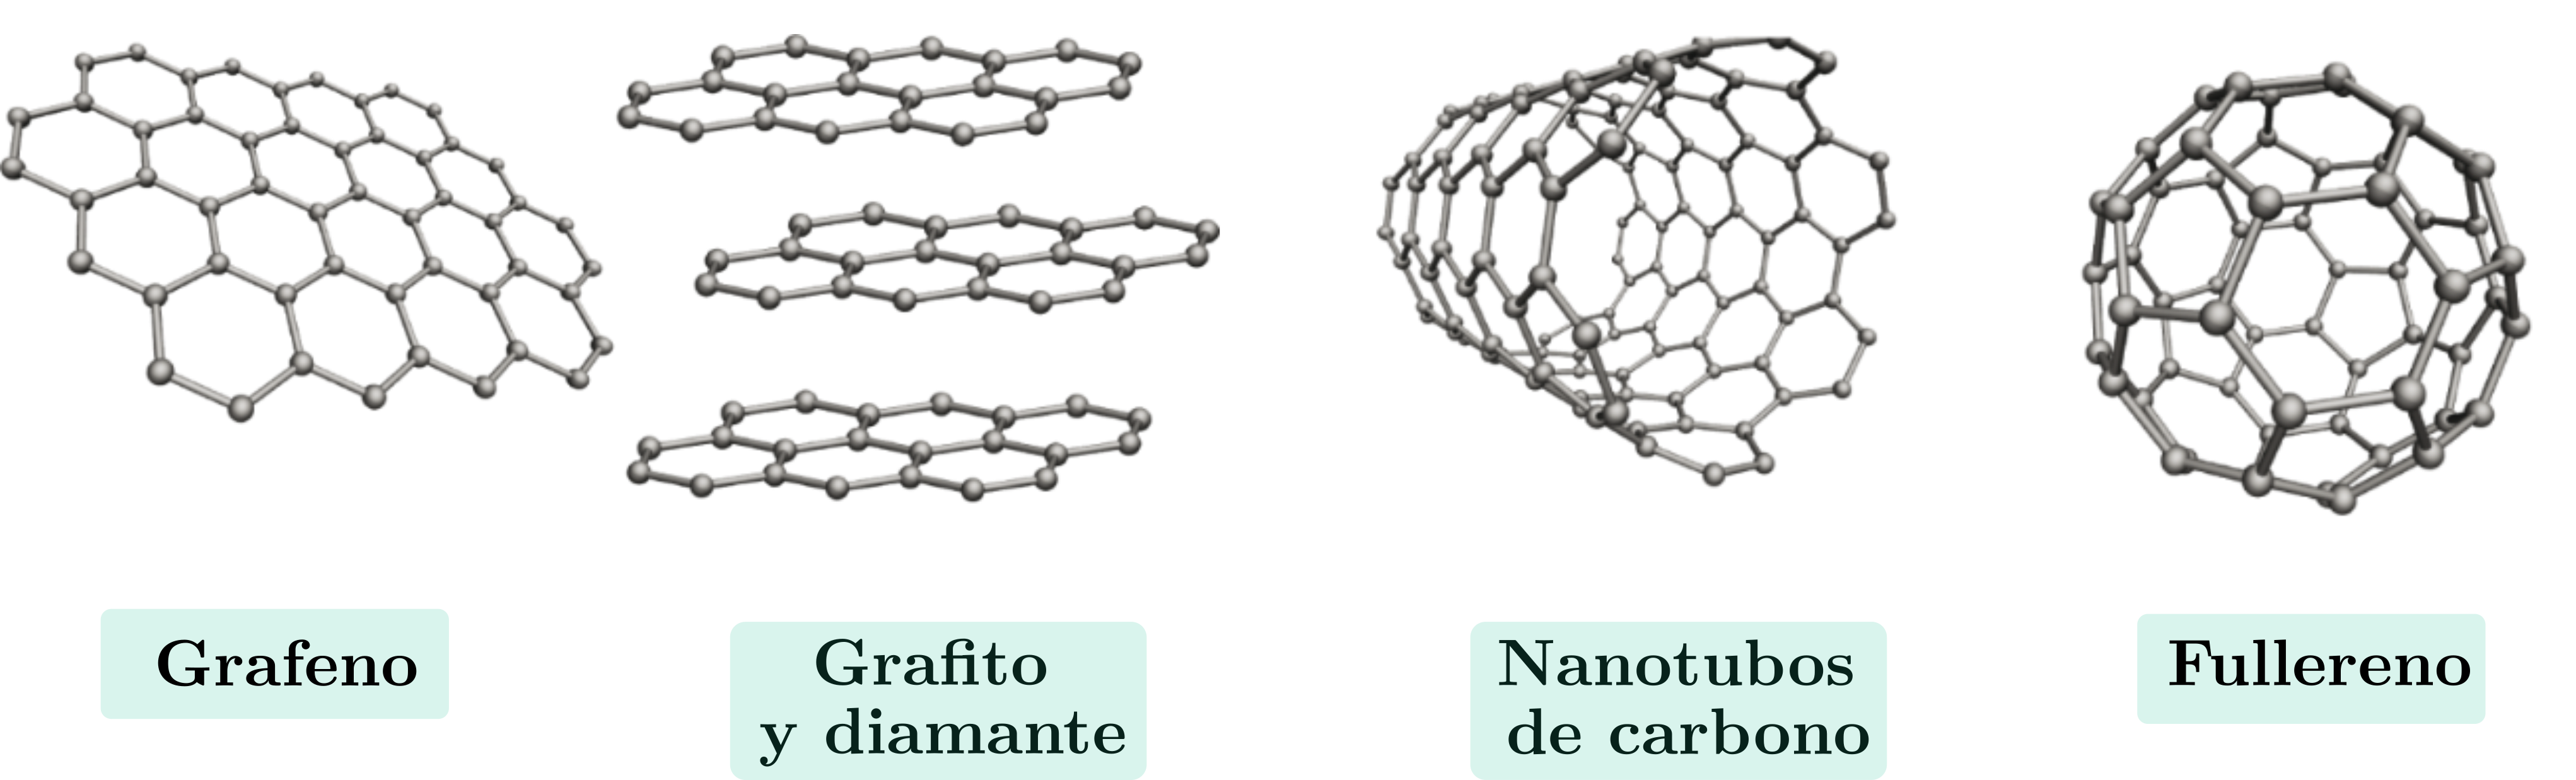
\includegraphics[width=\textwidth]{imagenes/Ant/alotropos.png}
  \caption{Representación esquemática de las principales formas alotrópicas del carbono \cite{medrano2012grafeno}.}
  \label{fig:alotropos-carbono}
\end{figure}

\subsection{Historia y Descubrimiento}
El descubrimiento del primer fulereno ocurrió en septiembre de 1985 en la Universidad Rice. Fue el resultado de una colaboración entre Harold Kroto (de la Universidad de Sussex), Robert Curl y Richard Smalley, quienes recibieron el Premio Nobel de Química en 1996 por este hallazgo. Inicialmente, el interés de Kroto se centraba en el análisis espectral de cadenas de carbono en el medio interestelar y su síntesis en el laboratorio. Para recrear estas condiciones, empleó un equipo de ablación láser diseñado para generar cúmulos atómicos, el cual simulaba la atmósfera de ciertas estrellas gigantes rojas. Al analizar los productos mediante espectrometría de masas por tiempo de vuelo, el equipo detectó una señal dominante a los 47 microsegundos. Esta señal equivalía a una masa atómica de 720 unidades (u), correspondiente a 60 átomos de carbono. La molécula mostró una estabilidad excepcional, formándose de manera preferente bajo las condiciones experimentales adecuadas \cite{martinez2024emergence}.

En el procedimiento experimental, se empleó un haz láser pulsado de alta potencia para calentar un disco de grafito y generar vapor de carbono. Este vapor fue arrastrado por un flujo de helio hacia una zona de expansión para condensar los átomos en cúmulos. Posteriormente, tras enfriarse y colimarse mediante una rendija, el flujo se analizó en el espectrómetro de masas. El experimento confirmó la presencia destacada de la especie de 720 u (C\textsubscript{60}). Aunque los datos iniciales no revelaban directamente su configuración tridimensional, la elevada estabilidad de la molécula llevó a los científicos a proponer una estructura esférica basada en el diseño de una cúpula geodésica \cite{poole2007introduccion}.

Junto al pico principal del C\textsubscript{60}, las pruebas espectrométricas detectaron una señal menor a 840 u.m.a., atribuida a la molécula de C\textsubscript{70}. A partir de estos hallazgos, se propuso que el C\textsubscript{60} es una nanoestructura carbonosa compuesta por 60 átomos organizados en una jaula cerrada de geometría icosaédrica simétrica, donde todos los átomos de carbono son equivalentes \textbf{véase la Figura \ref{fig:jaula-c60}}. Más adelante, en 1990, Krätschmer y colaboradores, en el Instituto Max Planck, desarrollaron un método de síntesis a gran escala mediante descargas de arco eléctrico entre electrodos de grafito en atmósfera de helio. Este proceso permitía obtener un hollín rico en fulerenos, del cual se logró aislar e identificar el C\textsubscript{60} mediante extracción con tolueno \cite{andrada2012nanotecnologia, liu2024quantum, garcia2023sintesis}. 

\begin{figure}[H]
  \centering
  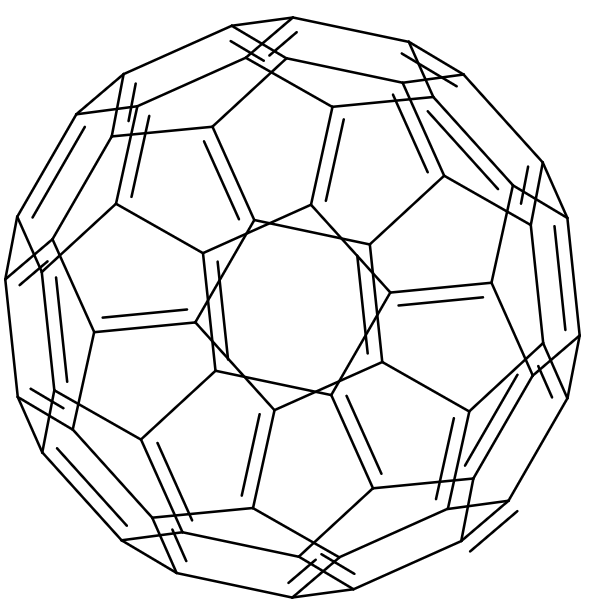
\includegraphics[width=6cm]{imagenes/Ant/c60.png}
  \caption{Representación esquemática del fulereno C\textsubscript{60}}
  \label{fig:jaula-c60}
\end{figure}


En la actualidad se reconoce que los fulerenos también se forman de manera natural en diversos procesos de alta temperatura que involucran materia carbonosa. Dado que las metodologías de síntesis masiva generan inevitablemente una mezcla heterogénea de fulerenos y otras nanoestructuras de carbono, el desarrollo tecnológico actual se enfoca en maximizar el rendimiento del hollín sintetizado, así como en optimizar los procesos de separación y purificación de especies específicas \cite{cavina2024orthoflaviviral}.


\subsection{Propiedades Fisicoquímicas y Estructura Cristalina del C\textsubscript{60}}

Los fulerenos son alótropos del carbono estructurados como poliedros huecos, esféricos u ovoides. Su nombre rinde homenaje a las cúpulas geodésicas de Sir R. Buckminster Fuller. El representante más común es el C\textsubscript{60} (buckminsterfulereno), una molécula con geometría de icosaedro truncado constituida por 60 vértices y 32 caras (20 hexagonales y 12 pentagonales) \textbf{véase la Figura \ref{fig:estructura-c60}}. En esta arquitectura, cada átomo de carbono presenta hibridación $sp^2$ y coordinación trigonal. La distancia media del enlace C--C, determinada mediante resonancia magnética nuclear (RMN), es de $1.44\ \text{\AA}$. Por su parte, los cuatro electrones de valencia de cada carbono forman dos enlaces simples y uno doble rico en electrones. Al satisfacer sus capas de valencia, el empaquetamiento molecular genera un sólido cristalino de van der Waals con propiedades aislantes o semiconductoras \cite{wilson2024role}.

\begin{figure}[H]
  \centering
  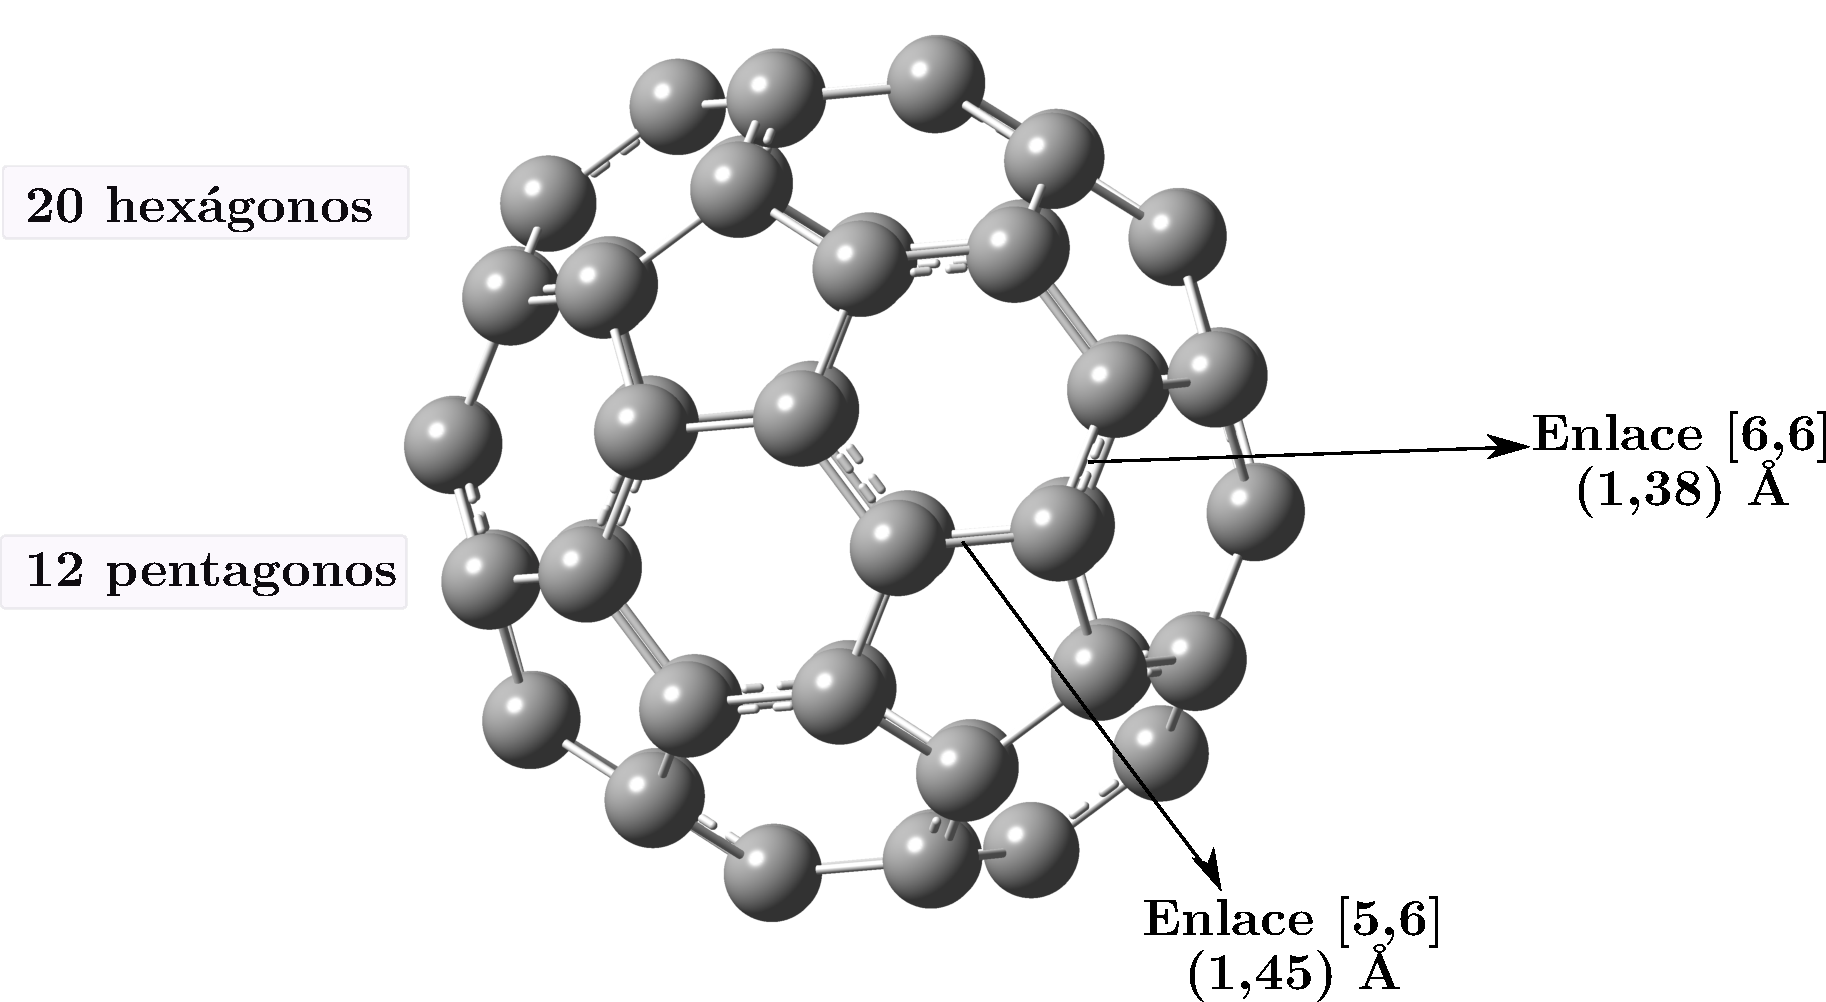
\includegraphics[width=15cm]{imagenes/Ant/c60.pdf}
  \caption{Estructura del C\textsubscript{60}: distribución de pentágonos y hexágonos y distinción entre enlaces [5,6] y [6,6].}
  \label{fig:estructura-c60}
\end{figure}

En términos dimensionales, esta molécula posee un diámetro externo promedio de $0.7\text{ nm}$. Asimismo, está constituida por anillos aromáticos condensados que conforman un sistema $\pi$ totalmente extendido y conjugado \cite{nakamura2012water}.

La conformación de la jaula cerrada del C\textsubscript{60} requiere combinar caras pentagonales y hexagonales, principio sustentado por el teorema de Euler. Este teorema establece que se necesitan exactamente 12 pentágonos para cerrar la red polimérica, sin importar el número de hexágonos incorporados. Como los anillos pentagonales introducen una elevada tensión angular en la red de enlaces, la presencia de pentágonos adyacentes desestabiliza la estructura. Este fenómeno se formaliza en la Regla del Pentágono Aislado (IPR). Por esta razón, el C\textsubscript{60} representa la estructura más pequeña que alberga 12 pentágonos sin compartir aristas. No obstante, en los espectros de masas iniciales se detectó una señal destacada de C\textsubscript{28} (12 pentágonos y solo 2 hexágonos). A pesar de infringir la regla IPR, esta especie presenta una configuración electrónica inusualmente estable \cite{cavina2024orthoflaviviral}.

Debido a la elevada densidad de dobles enlaces disponibles para reaccionar con radicales libres, la estructura del C\textsubscript{60} se ha investigado ampliamente para aplicaciones biomédicas. Esta molécula exhibe propiedades antioxidantes excepcionales y cuenta con la capacidad de atravesar membranas celulares y la barrera hematoencefálica. Asimismo, logra modular el transporte iónico y presenta afinidad interfacial con bicapas lipídicas \cite{norshidah2023assessing}.

Por otra parte, una propiedad crítica en el diseño farmacológico es la lipofilia, la cual se evalúa mediante el coeficiente de reparto octanol-agua ($\log P_{\text{ow}}$). En este sentido, el C\textsubscript{60} prístino no modificado es altamente lipofílico, registrando un valor de $\log P_{\text{ow}} = 6.67$ \cite{sharoyko2021biologically}.

Como consecuencia de esta elevada lipofilia, las moléculas de fulereno puro son fuertemente hidrófobas. Por ello, resultan prácticamente insolubles en medios acuosos y fluidos biológicos \cite{marforio2021dissecting}.
\section{Estrategias de Funcionalización Química}

La funcionalización superficial de los nanomateriales de carbono (CNM) constituye una estrategia fundamental para optimizar su biodegradabilidad, perfil de seguridad y solubilidad en medios acuosos. La modificación de la superficie de los CNM permite generar un sistema dinámico al combinar diversos fármacos, péptidos, ácidos nucleicos, aminoácidos y proteínas. Este anclaje estratégico incrementa la eficiencia farmacológica y la solubilidad del compuesto, reduciendo de manera simultánea su citotoxicidad intrínseca. La incorporación de estos agentes funcionales se realiza mediante interacciones intermoleculares covalentes o no covalentes (iónicas, fuerzas de van der Waals y apilamiento $\pi$--$\pi$). Esta disposición facilita la localización dirigida en regiones específicas de la arquitectura nanométrica \cite{gaur2021biomedical}.

Por su parte, los fulerenos constituyen una familia de materiales hidrofóbicos integrados exclusivamente por átomos de carbono dispuestos en forma de poliedros huecos \cite{sharoyko2021biologically}. % Nota bibliográfica original pendiente de correspondencia: (18)
 Desde su aislamiento en 1990, la química de los fulerenos ha experimentado una profunda evolución. De este modo, se ha demostrado su capacidad para interactuar con diversos solutos en entornos ambientales y sistemas biológicos, ejerciendo efectos significativos sobre el metabolismo, el transporte y la reactividad celular \cite{ chang2024recent, bai2024research}. Sin embargo, la molécula de C\textsubscript{60} carece intrínsecamente de una solubilidad acuosa adecuada ($< 10^{-11}\ \text{g/L}$), lo que induce su rápida agregación coloidal en medios fisiológicos. Para superar esta limitación crítica se emplean principalmente dos metodologías \cite{sosnowska2019mechano}:

\begin{itemize}
    \item \textbf{Complejación no covalente:} Utilización de agentes solubilizantes para enmascarar parcialmente la superficie hidrófoba de la jaula de carbono.
    \item \textbf{Funcionalización covalente:} Modificación química directa sobre los dobles enlaces de la superficie del fulereno.
\end{itemize}

En este contexto, la síntesis de derivados de fulereno (FD) mediante la adhesión covalente de fracciones hidrofílicas se ve favorecida por la elevada curvatura del C\textsubscript{60} y su extenso sistema de electrones $\pi$ conjugados. Esta elevada reactividad química permite acoplar cadenas laterales hidrofílicas, anfifílicas o estructuras de anillos fusionados al núcleo esférico, transformando a los fulerenos en versátiles bloques de construcción nanométricos. Al incorporar estas cadenas, los derivados pueden conservar o potenciar su capacidad para generar oxígeno singlete ($^1\text{O}_2$), radicales hidroxilo ($\cdot\text{OH}$) y aniones superóxido ($\text{O}_2^{\bullet-}$). Asimismo, este proceso incrementa el momento dipolar y favorece la estabilidad coloidal en disolventes polares \cite{gaur2021biomedical}.

Se ha establecido que los derivados del C\textsubscript{60} poseen energías de reorganización sumamente pequeñas durante los procesos de transferencia electrónica. Esta propiedad los convierte en aceptores de electrones ideales para aplicaciones biomédicas y energéticas. \cite{sharoyko2021biologically, nelson2022principios}. En los últimos años, el desarrollo de enfoques sintéticos avanzados ha permitido obtener aductos de fulereno con solubilidades acuosas fisiológicamente aceptables, alcanzando concentraciones de entre 10 y $200\ \text{mg/mL}$ o superiores. % Nota bibliográfica original pendiente de correspondencia: (28)
 Gracias a estas características, los fulerenos funcionalizados destacan en cosmetología, ciencia de materiales, electroquímica y sistemas de liberación controlada de fármacos \cite{andrada2012nanotecnologia, liu2024quantum}. La diversificación de sus aductos solubles en agua incluye fulerenoles, carboxifulerenos y conjugados con aminoácidos. Estos compuestos destacan por presentar actividad antioxidante, antimicrobiana, neuroprotectora, radioprotectora, así como su uso como fotosensibilizadores en terapia fotodinámica e inhibidores enzimáticos \cite{marforio2021dissecting}.

\subsubsection{Fulereno con Glicina (C\textsubscript{60}--Gly): Síntesis y Caracterización Estructural}

A diferencia de otros aminoácidos estándar cuyo carbono $\alpha$ constituye un centro quiral, la glicina (Gly) es el aminoácido estructuralmente más simple y carece de quiralidad. Aunque formalmente se clasifica como apolar, su diminuta cadena lateral —constituida por un único átomo de hidrógeno— no genera impedimento estérico ni aporta una contribución hidrofóbica significativa \cite{bolshakova2023facile}. Por su parte, los conjugados de fulereno con aminoácidos (fulleroaminoácidos) resultan de elevado interés biomédico. Esto se debe a que la fracción funcionalizadora aporta hidrofilia y biocompatibilidad, al tiempo que conserva importantes actividades biológicas útiles en la administración de fármacos antitumorales, neuroprotectores, antioxidantes y antivirales \cite{jiang2015synthesis}.

Los aminoácidos destacan como ligandos idóneos para modificar la jaula de C\textsubscript{60} gracias a la presencia de sus grupos polares carboxilo (--COOH) y amino (--NH\textsubscript{2}). En el caso de la glicina, su reducido volumen molecular minimiza el impedimento estérico. Al mismo tiempo, la elevada nucleofilia de su grupo amino terminal facilita su unión mediante un ataque nucleofílico directo sobre los dobles enlaces electrófilos del C\textsubscript{60} \textbf{véase la Figura \ref{Fig:molecula}}\cite{jiang2015synthesis}. Recientemente, se reportó la síntesis del aducto tetrasustituido de C\textsubscript{60} funcionalizado con glicina, denominado C\textsubscript{60}--Gly [C\textsubscript{60}(C\textsubscript{2}H\textsubscript{4}NO\textsubscript{2})\textsubscript{4}], el cual alcanzó un rendimiento sintético del 85\% y una pureza cromatográfica del 99.8\%. % Nota bibliográfica original pendiente de correspondencia: (50)
 La Figura~\ref{Fig:molecula} representa la estructura química del aducto C\textsubscript{60}--Gly. 

\begin{figure}[H]
  \centering
  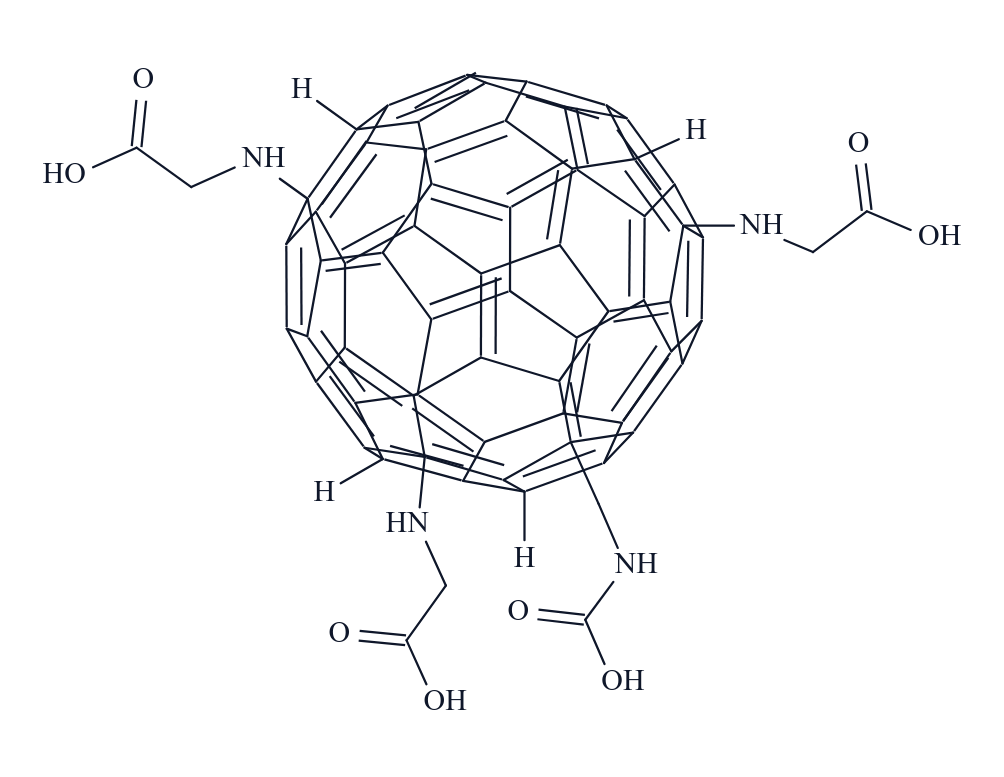
\includegraphics[width=11cm]{imagenes/Resu/molecula.png}
  \caption{Estructura del C\textsubscript{60} funcionalizado con 4 aminoácidos de glicina.}
  \label{Fig:molecula}
\end{figure}

% Nota bibliográfica original pendiente de correspondencia: (50)
 La caracterización espectroscópica de la Figura~\ref{Fig:rmn_c60_gly}, mediante resonancia magnética nuclear de carbono-13 (\textsuperscript{13}C RMN) confirma de manera inequívoca el enlace covalente a la jaula esférica. El espectro de \textsuperscript{13}C RMN del aducto C\textsubscript{60}--Gly exhibe desplazamientos químicos característicos a $177\text{ ppm}$ ($a$, carbono carboxílico), $144\text{ ppm}$ (núcleo de $sp^2$-C\textsubscript{60}), $65\text{ ppm}$ ($c$, $sp^3$-C de la jaula enlazado al grupo amino), $50\text{ ppm}$ ($b$, grupo metileno --CH\textsubscript{2}--) y $17\text{ ppm}$ ($d$, $sp^3$-C unido a hidrógeno). 

\begin{figure}[H]
  \centering
  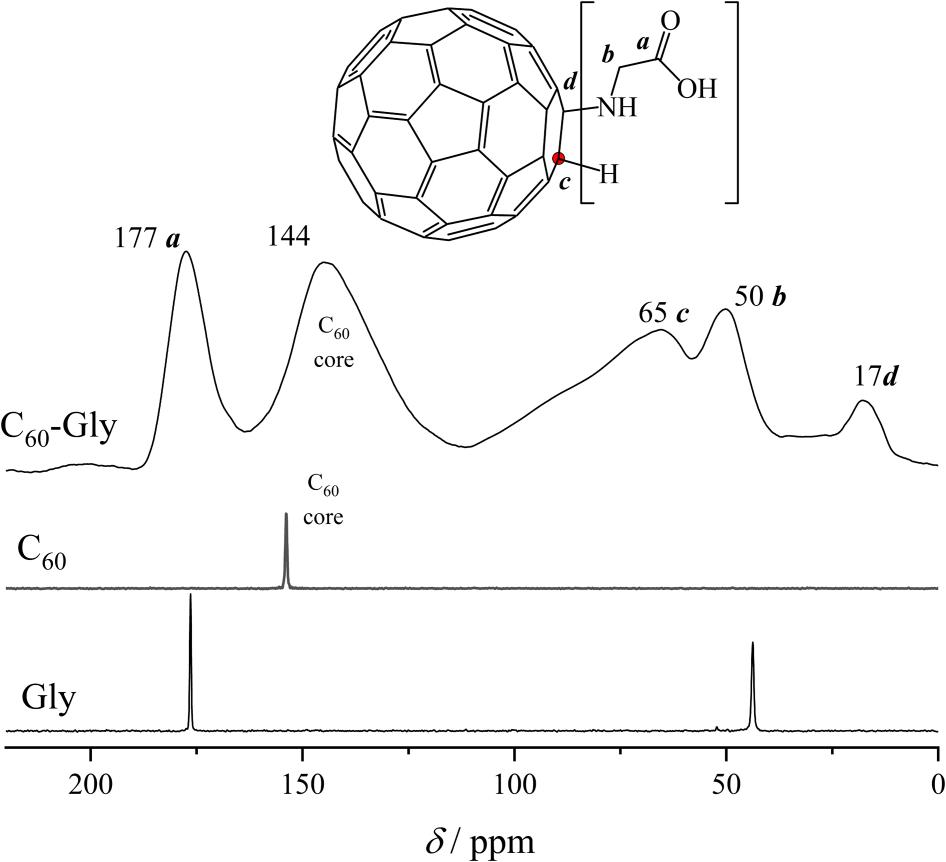
\includegraphics[width=11cm]{imagenes/Ant/NMR.png}
  \caption{Espectro de RMN de \textsuperscript{13}C y asignación de señales estructurales del aducto C\textsubscript{60}--Gly.}
  \label{Fig:rmn_c60_gly}
\end{figure}

Desde la perspectiva fisicoquímica, el aducto C\textsubscript{60}--Gly presenta un coeficiente de partición de $\log P_{\text{ow}} = 0.25$. Este valor evidencia una afinidad equilibrada tanto por fases acuosas como lipídicas, lo que contrasta con la extrema hidrofobicidad del C\textsubscript{60} prístino ($\log P_{\text{ow}} = 6.67$). % Nota bibliográfica original pendiente de correspondencia: (50)
 En disolución acuosa, el aducto se autoasocia en nanoagregados coloidales de 30 a $50\text{ nm}$ con un potencial zeta ($\zeta$) de $-40$ a $-30\text{ mV}$, lo que asegura una elevada estabilidad coloidal por repulsión electrostática \cite{sharoyko2024modification}. Sus principales propiedades y parámetros estructurales se resumen en la Tabla~\ref{tab:aplicaciones_fulereno}. \cite{nakamura2012water,jiang2015synthesis,sharoyko2024modification}.

\begin{table}[H]
\centering
\caption{Propiedades fisicoquímicas y estructurales del aducto C\textsubscript{60}--Gly (Fulereno--Glicina) para aplicaciones biomédicas.}
\label{tab:aplicaciones_fulereno}
\begin{tabular}{l p{10cm}}
\toprule
\textbf{Característica / Parámetro} & \textbf{Descripción del aducto C\textsubscript{60}--Gly} \\
\midrule
Estequiometría y pureza & Tetraaducto C\textsubscript{60}(C\textsubscript{2}H\textsubscript{4}NO\textsubscript{2})\textsubscript{4} (Rendimiento: 85\%, Pureza: 99.8\%).\\
Geometría del ligando & Sin cadena lateral voluminosa; impedimento estérico mínimo. \\
Grupos funcionales terminales & Grupos carboxilo y grupos nitrogenados asociados con la unión de glicina a la jaula. \\
Perfil de lipofilia ($\log P_{\text{ow}}$) & $\log P_{\text{ow}} = 0.25$ (carácter anfifílico equilibrado). \\
Comportamiento coloidal & Nanoasociados ($30\text{--}50\text{ nm}$) con alta estabilidad ($\zeta = -40\text{ a }-30\text{ mV}$). \\
Seguridad biológica & Alta hemocompatibilidad, baja citotoxicidad e inhibición de agregación plaquetaria  \cite{sharoyko2024modification}. \\
\bottomrule
\end{tabular}
\end{table}

La superficie del fulereno prístino presenta regiones con deficiencia electrónica (agujeros $\pi$), las cuales establecen interacciones anión--$\pi$ con residuos cargados negativamente. Asimismo, interactúa mediante apilamiento $\pi$--$\pi$ con residuos aromáticos (Trp, Phe, Tyr, His) y mediante interacciones hidrofóbicas con residuos alifáticos (Leu, Val, Pro, Ile, Ala, Met). Por su parte, las cadenas laterales catiónicas (Arg, Lys) forman interacciones catión--$\pi$ sustancialmente más fuertes que los residuos neutros (Asn, Gln). Adicionalmente, la densidad electrónica de la jaula le permite actuar como aceptor de puentes de hidrógeno no estándar. % Nota bibliográfica original pendiente de correspondencia: (30)
 Los principales tipos de interacciones intermoleculares se resumen a continuación (véase la Tabla~\ref{tab:interacciones_fulereno}) \cite{bolshakova2023facile}.

\begin{table}[H]
\centering
\caption{Principales tipos de interacciones intermoleculares entre la superficie de fulerenos y residuos aminoacídicos en estructuras proteicas.}
\label{tab:interacciones_fulereno}
\begin{tabular}{l l}
\toprule
\textbf{Tipo de Interacción} & \textbf{Mecanismo / Residuos Involucrados} \\
\midrule
Apilamiento $\pi$--$\pi$ & Residuos aromáticos (Trp, Phe, Tyr, His) \\
Interacciones hidrofóbicas & Residuos alifáticos (Leu, Val, Pro, Ile, Ala, Met) \\
Interacciones catión--$\pi$ & Cadenas con carga positiva (Arg, Lys) \\
Interacciones anión--$\pi$ & Residuos cargados negativamente / Agujeros $\pi$ \\
Puentes de hidrógeno & Enlaces no estándar en regiones ricas en $e^-$ \\
Efecto tipo surfactante & Cadenas anfifílicas y polares \\
\bottomrule
\end{tabular}
\end{table}

\section{Química Cuántica y Teoría del Funcional de la Densidad (DFT)}
La Teoría del Funcional de la Densidad (DFT) se fundamenta en que la densidad electrónica del estado fundamental, $\rho(\vec{r})$, es la variable fundamental para describir la energía y las propiedades electrónicas de un sistema multielectrónico en su estado fundamental. En este marco formal, la energía total del sistema $E[\rho]$ se expresa como un funcional de $\rho(\vec{r})$, donde el término de intercambio y correlación $E_{\text{xc}}[\rho]$ compensa las diferencias de energía cinética e interacciones interelectrónicas entre el sistema real interactuante y un sistema de referencia ficticio de electrones no interactuantes (Kohn-Sham). Por su parte, el modelado \textit{in silico} mediante DFT permite optimizar la geometría molecular ajustando las coordenadas atómicas —como longitudes, ángulos de enlace y ángulos de torsión— hasta lograr la minimización de la superficie de energía potencial \cite{kohn1965self}.

Para el estudio de aductos de fulereno C\textsubscript{60} funcionalizados con aminoácidos, la elección del funcional y la base es determinante para equilibrar el costo computacional y la precisión electrónica. El funcional híbrido B3LYP combina el intercambio exacto de Hartree-Fock con los funcionales de intercambio de Becke (B3) y la correlación de Lee-Yang-Parr (LYP), estando ampliamente validado para la caracterización de nanoestructuras carbonosas. Por otro lado, el conjunto de bases polarizado triple-zeta 6-311G(d,p) emplea 6 funciones gaussianas primitivas para los electrones del núcleo (\textit{core}) y triplica la descripción de los orbitales de valencia, añadiendo funciones $d$ en átomos pesados y $p$ en átomos de hidrógeno. Esta combinación resulta idónea para mapear transferencias de carga, momentos dipolares y densidades electrónicas en intermediarios monocarboxilados y poliderivados \cite{nikolaev2020thermodynamic, mico2024estudio}.

 Mediante una aproximación basada en los orbitales frontera, los niveles energéticos del orbital ocupado de mayor energía ($E_{\text{HOMO}}$) y del orbital desocupado de menor energía ($E_{\text{LUMO}}$) permiten cuantificar los descriptores globales de reactividad química. El potencial de ionización ($I$) y la afinidad electrónica ($A$) se aproximan según:
\begin{equation}
I \approx -E_{\text{HOMO}}
\end{equation}
\begin{equation}
A \approx -E_{\text{LUMO}}
\end{equation}

Asimismo, la DFT permite explorar la reactividad local de una molécula a través de las funciones de Fukui (FF). Estas funciones, derivadas mediante esquemas de diferencias finitas ($\Delta N = \pm 1$), identifican los sitios atómicos propensos a ataques nucleofílicos ($f^+$), electrófilos ($f^-$) o por radicales libres ($f^0$):
\begin{equation}
f^+(\vec{r}) = \rho_{\text{anión}}(\vec{r}) - \rho_{\text{neutro}}(\vec{r}) \quad \text{(Ataque nucleofílico / Regiones electrófilas)}
\end{equation}
\begin{equation}
f^-(\vec{r}) = \rho_{\text{neutro}}(\vec{r}) - \rho_{\text{catión}}(\vec{r}) \quad \text{(Ataque electrófilo / Regiones nucleofílicas)}
\end{equation}
\begin{equation}
f^0(\vec{r}) = \frac{\rho_{\text{anión}}(\vec{r}) - \rho_{\text{catión}}(\vec{r})}{2} \quad \text{(Ataque por radicales libres)}
\end{equation}
Las aproximaciones orbitales para $I$ y $A$ no equivalen a diferencias de energía total. Las definiciones y sus limitaciones se desarrollan en los Apéndices~\ref{ap:fundamentos-gaussian} y \ref{ap:reactividad}.

En aductos de C\textsubscript{60} funcionalizados con aminoácidos (como L-arginina o glicina), los cálculos indican que los átomos de carbono del núcleo enlazados al aminoácido ceden densidad electrónica hacia los átomos de nitrógeno adyacentes. Este reordenamiento polariza localmente la jaula, permitiendo la formación de interacciones intermoleculares selectivas tanto por el núcleo hiperconjugado como por las cadenas laterales de los residuos \cite{moncada2008caracterizacion, gaur2021biomedical}.

\subsection{Acoplamiento molecular, dinámica molecular y evaluación de actividad biomédica}
El acoplamiento molecular permite predecir los modos de unión óptimos y las afinidades de enlace entre aductos de fulereno y dianas proteicas de relevancia clínica. Empleando herramientas como AutoDock Vina, se parametrizan rejillas tridimensionales (cajas de delimitación) centradas en bolsillos catalíticos o alostéricos. De este modo, se evalúan formas abiertas y cerradas de enzimas clave como la proteasa NS2B-NS3 del virus del dengue (DENV-2), la proteína tirosina fosfatasa 1B (PTP1B) o la proteasa del VIH-1. Las interacciones se estabilizan mediante el acomodamiento hidrofóbico de la jaula en la cavidad no polar, interacciones catión--$\pi$ con cadenas laterales básicas (Arg, Lys) y puentes de hidrógeno dirigidos por las fracciones carboxilo y amino terminales del aminoácido acoplado \cite{nelson2022principios,jiang2015synthesis, wang2024strain}.

Por su parte, la dinámica molecular (DM) profundiza en la estabilidad temporal y la flexibilidad conformacional de los complejos ligando-proteína. Utilizando entornos de cómputo como GROMACS y campos de fuerza como GROMOS96 (53A6) —con topologías de ligando parametrizadas vía servidores como ATB y cargas atómicas cuánticas—, el sistema se solvata en modelos de agua explícita (por ejemplo, SPC) e iones de neutralización ($\text{Na}^+/\text{Cl}^-$). Tras la minimización energética por descenso más pronunciado, el sistema se somete a fases de equilibrado isocórico-isotérmico (NVT, $300\text{ K}$) e isotérmico-isobárico (NPT, $1.0\text{ bar}$) mediante acoplamientos de temperatura (V-rescale) y presión (Parrinello-Rahman). La energía libre de unión ($\Delta G_{\text{bind}}$) se cuantifica posteriormente a través de métodos de disolvente continuo (\textit{Continuum Solvent}) como MM/GBSA (\textit{Molecular Mechanics/Generalized Born Surface Area}) en paquetes como AMBER, desglosando las contribuciones entálpicas y electrostáticas residuo por residuo \cite{nelson2022principios, liu2023fullerene}.

La integración del modelado \textit{in silico} respalda de manera directa el potencial biomédico de los fulerenos funcionalizados en diversas patologías humanas. Gracias a su extensa red de electrones $\pi$, el C\textsubscript{60} funcionalizado actúa como una ``esponja de radicales libres'', atrapando especies reactivas de oxígeno (ROS) e inhibiendo el estrés oxidativo involucrado en el daño tisular y neurodegenerativo (enfermedades de Alzheimer y Parkinson). Asimismo, las simulaciones demuestran que las interacciones electrostáticas e hidrofóbicas entre los aductos hidrofílicos y los oligómeros del péptido $\beta$-amiloide ($\text{A}\beta$) o la $\alpha$-sinucleína alteran el autoensamblaje fibrilar, deteniendo la polimerización neurotóxica. En terapias fotodinámicas (PDT) y patógenos infecciosos, estos derivados generan la fotoinactivación de microorganismos y la rotura de membranas bacterianas, mostrando una biocompatibilidad dependiente de la dosis y de la arquitectura sintética del aducto \cite{wilson2024role, wang2024strain,  celaya2022administracion, partha2009biomedical}.
  


















